% Options for packages loaded elsewhere
\PassOptionsToPackage{unicode}{hyperref}
\PassOptionsToPackage{hyphens}{url}
\PassOptionsToPackage{dvipsnames,svgnames,x11names}{xcolor}
%
\documentclass[
  letterpaper,
  DIV=11,
  numbers=noendperiod]{scrartcl}

\usepackage{amsmath,amssymb}
\usepackage{iftex}
\ifPDFTeX
  \usepackage[T1]{fontenc}
  \usepackage[utf8]{inputenc}
  \usepackage{textcomp} % provide euro and other symbols
\else % if luatex or xetex
  \usepackage{unicode-math}
  \defaultfontfeatures{Scale=MatchLowercase}
  \defaultfontfeatures[\rmfamily]{Ligatures=TeX,Scale=1}
\fi
\usepackage{lmodern}
\ifPDFTeX\else  
    % xetex/luatex font selection
\fi
% Use upquote if available, for straight quotes in verbatim environments
\IfFileExists{upquote.sty}{\usepackage{upquote}}{}
\IfFileExists{microtype.sty}{% use microtype if available
  \usepackage[]{microtype}
  \UseMicrotypeSet[protrusion]{basicmath} % disable protrusion for tt fonts
}{}
\makeatletter
\@ifundefined{KOMAClassName}{% if non-KOMA class
  \IfFileExists{parskip.sty}{%
    \usepackage{parskip}
  }{% else
    \setlength{\parindent}{0pt}
    \setlength{\parskip}{6pt plus 2pt minus 1pt}}
}{% if KOMA class
  \KOMAoptions{parskip=half}}
\makeatother
\usepackage{xcolor}
\setlength{\emergencystretch}{3em} % prevent overfull lines
\setcounter{secnumdepth}{-\maxdimen} % remove section numbering
% Make \paragraph and \subparagraph free-standing
\ifx\paragraph\undefined\else
  \let\oldparagraph\paragraph
  \renewcommand{\paragraph}[1]{\oldparagraph{#1}\mbox{}}
\fi
\ifx\subparagraph\undefined\else
  \let\oldsubparagraph\subparagraph
  \renewcommand{\subparagraph}[1]{\oldsubparagraph{#1}\mbox{}}
\fi

\usepackage{color}
\usepackage{fancyvrb}
\newcommand{\VerbBar}{|}
\newcommand{\VERB}{\Verb[commandchars=\\\{\}]}
\DefineVerbatimEnvironment{Highlighting}{Verbatim}{commandchars=\\\{\}}
% Add ',fontsize=\small' for more characters per line
\usepackage{framed}
\definecolor{shadecolor}{RGB}{241,243,245}
\newenvironment{Shaded}{\begin{snugshade}}{\end{snugshade}}
\newcommand{\AlertTok}[1]{\textcolor[rgb]{0.68,0.00,0.00}{#1}}
\newcommand{\AnnotationTok}[1]{\textcolor[rgb]{0.37,0.37,0.37}{#1}}
\newcommand{\AttributeTok}[1]{\textcolor[rgb]{0.40,0.45,0.13}{#1}}
\newcommand{\BaseNTok}[1]{\textcolor[rgb]{0.68,0.00,0.00}{#1}}
\newcommand{\BuiltInTok}[1]{\textcolor[rgb]{0.00,0.23,0.31}{#1}}
\newcommand{\CharTok}[1]{\textcolor[rgb]{0.13,0.47,0.30}{#1}}
\newcommand{\CommentTok}[1]{\textcolor[rgb]{0.37,0.37,0.37}{#1}}
\newcommand{\CommentVarTok}[1]{\textcolor[rgb]{0.37,0.37,0.37}{\textit{#1}}}
\newcommand{\ConstantTok}[1]{\textcolor[rgb]{0.56,0.35,0.01}{#1}}
\newcommand{\ControlFlowTok}[1]{\textcolor[rgb]{0.00,0.23,0.31}{#1}}
\newcommand{\DataTypeTok}[1]{\textcolor[rgb]{0.68,0.00,0.00}{#1}}
\newcommand{\DecValTok}[1]{\textcolor[rgb]{0.68,0.00,0.00}{#1}}
\newcommand{\DocumentationTok}[1]{\textcolor[rgb]{0.37,0.37,0.37}{\textit{#1}}}
\newcommand{\ErrorTok}[1]{\textcolor[rgb]{0.68,0.00,0.00}{#1}}
\newcommand{\ExtensionTok}[1]{\textcolor[rgb]{0.00,0.23,0.31}{#1}}
\newcommand{\FloatTok}[1]{\textcolor[rgb]{0.68,0.00,0.00}{#1}}
\newcommand{\FunctionTok}[1]{\textcolor[rgb]{0.28,0.35,0.67}{#1}}
\newcommand{\ImportTok}[1]{\textcolor[rgb]{0.00,0.46,0.62}{#1}}
\newcommand{\InformationTok}[1]{\textcolor[rgb]{0.37,0.37,0.37}{#1}}
\newcommand{\KeywordTok}[1]{\textcolor[rgb]{0.00,0.23,0.31}{#1}}
\newcommand{\NormalTok}[1]{\textcolor[rgb]{0.00,0.23,0.31}{#1}}
\newcommand{\OperatorTok}[1]{\textcolor[rgb]{0.37,0.37,0.37}{#1}}
\newcommand{\OtherTok}[1]{\textcolor[rgb]{0.00,0.23,0.31}{#1}}
\newcommand{\PreprocessorTok}[1]{\textcolor[rgb]{0.68,0.00,0.00}{#1}}
\newcommand{\RegionMarkerTok}[1]{\textcolor[rgb]{0.00,0.23,0.31}{#1}}
\newcommand{\SpecialCharTok}[1]{\textcolor[rgb]{0.37,0.37,0.37}{#1}}
\newcommand{\SpecialStringTok}[1]{\textcolor[rgb]{0.13,0.47,0.30}{#1}}
\newcommand{\StringTok}[1]{\textcolor[rgb]{0.13,0.47,0.30}{#1}}
\newcommand{\VariableTok}[1]{\textcolor[rgb]{0.07,0.07,0.07}{#1}}
\newcommand{\VerbatimStringTok}[1]{\textcolor[rgb]{0.13,0.47,0.30}{#1}}
\newcommand{\WarningTok}[1]{\textcolor[rgb]{0.37,0.37,0.37}{\textit{#1}}}

\providecommand{\tightlist}{%
  \setlength{\itemsep}{0pt}\setlength{\parskip}{0pt}}\usepackage{longtable,booktabs,array}
\usepackage{calc} % for calculating minipage widths
% Correct order of tables after \paragraph or \subparagraph
\usepackage{etoolbox}
\makeatletter
\patchcmd\longtable{\par}{\if@noskipsec\mbox{}\fi\par}{}{}
\makeatother
% Allow footnotes in longtable head/foot
\IfFileExists{footnotehyper.sty}{\usepackage{footnotehyper}}{\usepackage{footnote}}
\makesavenoteenv{longtable}
\usepackage{graphicx}
\makeatletter
\def\maxwidth{\ifdim\Gin@nat@width>\linewidth\linewidth\else\Gin@nat@width\fi}
\def\maxheight{\ifdim\Gin@nat@height>\textheight\textheight\else\Gin@nat@height\fi}
\makeatother
% Scale images if necessary, so that they will not overflow the page
% margins by default, and it is still possible to overwrite the defaults
% using explicit options in \includegraphics[width, height, ...]{}
\setkeys{Gin}{width=\maxwidth,height=\maxheight,keepaspectratio}
% Set default figure placement to htbp
\makeatletter
\def\fps@figure{htbp}
\makeatother

\KOMAoption{captions}{tableheading}
\makeatletter
\makeatother
\makeatletter
\makeatother
\makeatletter
\@ifpackageloaded{caption}{}{\usepackage{caption}}
\AtBeginDocument{%
\ifdefined\contentsname
  \renewcommand*\contentsname{Table of contents}
\else
  \newcommand\contentsname{Table of contents}
\fi
\ifdefined\listfigurename
  \renewcommand*\listfigurename{List of Figures}
\else
  \newcommand\listfigurename{List of Figures}
\fi
\ifdefined\listtablename
  \renewcommand*\listtablename{List of Tables}
\else
  \newcommand\listtablename{List of Tables}
\fi
\ifdefined\figurename
  \renewcommand*\figurename{Figure}
\else
  \newcommand\figurename{Figure}
\fi
\ifdefined\tablename
  \renewcommand*\tablename{Table}
\else
  \newcommand\tablename{Table}
\fi
}
\@ifpackageloaded{float}{}{\usepackage{float}}
\floatstyle{ruled}
\@ifundefined{c@chapter}{\newfloat{codelisting}{h}{lop}}{\newfloat{codelisting}{h}{lop}[chapter]}
\floatname{codelisting}{Listing}
\newcommand*\listoflistings{\listof{codelisting}{List of Listings}}
\makeatother
\makeatletter
\@ifpackageloaded{caption}{}{\usepackage{caption}}
\@ifpackageloaded{subcaption}{}{\usepackage{subcaption}}
\makeatother
\makeatletter
\@ifpackageloaded{tcolorbox}{}{\usepackage[skins,breakable]{tcolorbox}}
\makeatother
\makeatletter
\@ifundefined{shadecolor}{\definecolor{shadecolor}{rgb}{.97, .97, .97}}
\makeatother
\makeatletter
\makeatother
\makeatletter
\makeatother
\ifLuaTeX
  \usepackage{selnolig}  % disable illegal ligatures
\fi
\IfFileExists{bookmark.sty}{\usepackage{bookmark}}{\usepackage{hyperref}}
\IfFileExists{xurl.sty}{\usepackage{xurl}}{} % add URL line breaks if available
\urlstyle{same} % disable monospaced font for URLs
\hypersetup{
  pdftitle={Class05: Data visualization with ggplot},
  pdfauthor={Yi-Hung Lee (PID: A16587141)},
  colorlinks=true,
  linkcolor={blue},
  filecolor={Maroon},
  citecolor={Blue},
  urlcolor={Blue},
  pdfcreator={LaTeX via pandoc}}

\title{Class05: Data visualization with ggplot}
\author{Yi-Hung Lee (PID: A16587141)}
\date{}

\begin{document}
\maketitle
\ifdefined\Shaded\renewenvironment{Shaded}{\begin{tcolorbox}[borderline west={3pt}{0pt}{shadecolor}, breakable, interior hidden, boxrule=0pt, frame hidden, enhanced, sharp corners]}{\end{tcolorbox}}\fi

\renewcommand*\contentsname{Table of contents}
{
\hypersetup{linkcolor=}
\setcounter{tocdepth}{3}
\tableofcontents
}
\hypertarget{ggplot-introduction}{%
\subsection{ggplot introduction}\label{ggplot-introduction}}

Today we will have our first play with the \textbf{ggplot2} package -
one of the most popular graphics packages on the planet.

There are many plotting systems in R. These include so-called
\emph{``base''} plot/graphs.

Base plot is generally rather short code and dull plots - but it is
always for you and is fast for big dataset.

\begin{Shaded}
\begin{Highlighting}[]
\FunctionTok{plot}\NormalTok{(cars)}
\end{Highlighting}
\end{Shaded}

\begin{figure}[H]

{\centering 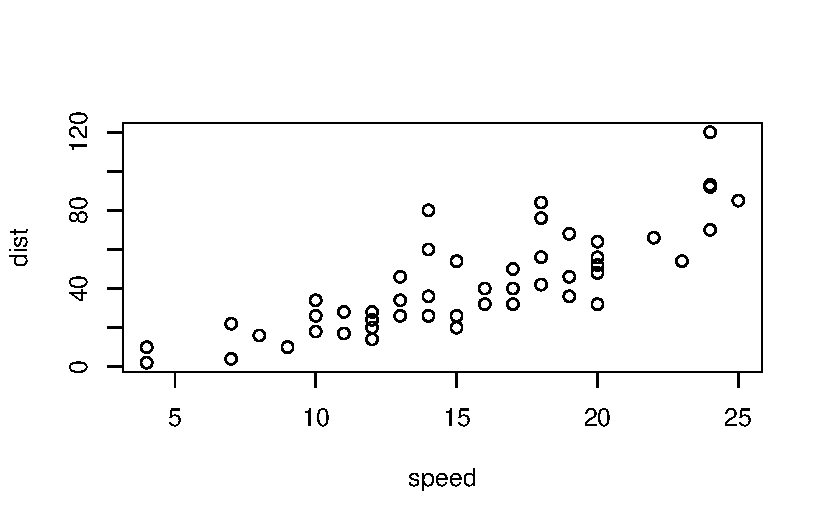
\includegraphics{class05_files/figure-pdf/unnamed-chunk-1-1.pdf}

}

\end{figure}

Try ggplot: Need to install \textbf{ggplot} package, use function
\texttt{install.packages()}. Already installed.

Every time I want to use a package, I need to call the library by
function \texttt{library(ggplot2)}

\begin{Shaded}
\begin{Highlighting}[]
\FunctionTok{library}\NormalTok{(ggplot2)}

\FunctionTok{ggplot}\NormalTok{(cars)}
\end{Highlighting}
\end{Shaded}

\begin{figure}[H]

{\centering 
\includegraphics{class05_files/figure-pdf/unnamed-chunk-2-1.pdf}

}

\end{figure}

Every \textbf{ggplot} has at least 3 things:

\begin{itemize}
\tightlist
\item
  \textbf{data}: the data. frame with the data you want to plot
\item
  \textbf{aes}: the aesthetic mapping of the data to the plot
\item
  \textbf{geom}: how do you want the plot to look
\end{itemize}

\begin{Shaded}
\begin{Highlighting}[]
\FunctionTok{ggplot}\NormalTok{(cars) }\SpecialCharTok{+}
  \FunctionTok{aes}\NormalTok{(}\AttributeTok{x=}\NormalTok{speed, }\AttributeTok{y=}\NormalTok{dist)}
\end{Highlighting}
\end{Shaded}

\begin{figure}[H]

{\centering 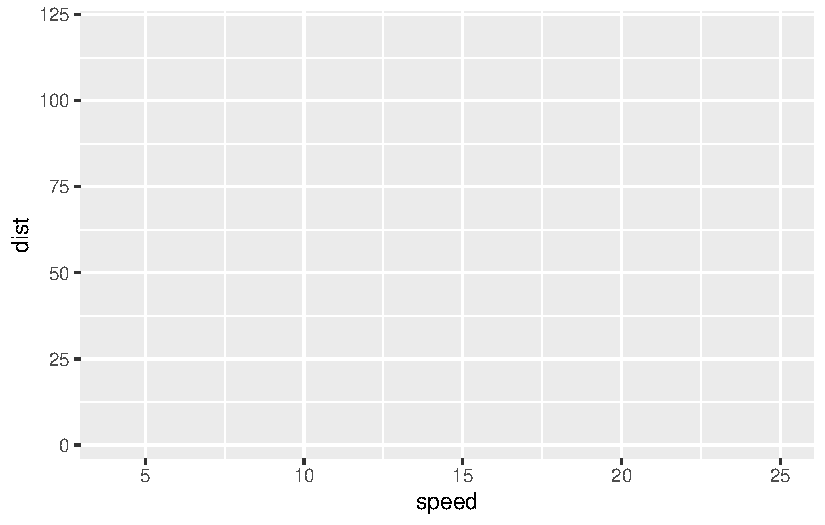
\includegraphics{class05_files/figure-pdf/unnamed-chunk-3-1.pdf}

}

\end{figure}

\begin{Shaded}
\begin{Highlighting}[]
\FunctionTok{ggplot}\NormalTok{(cars) }\SpecialCharTok{+}
  \FunctionTok{aes}\NormalTok{(}\AttributeTok{x =}\NormalTok{ speed, }\AttributeTok{y =}\NormalTok{ dist) }\SpecialCharTok{+}
  \FunctionTok{geom\_point}\NormalTok{()}
\end{Highlighting}
\end{Shaded}

\begin{figure}[H]

{\centering 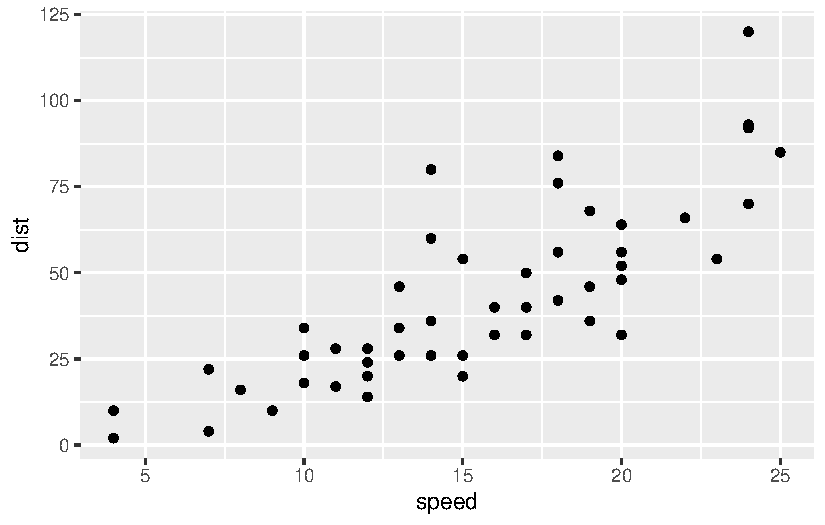
\includegraphics{class05_files/figure-pdf/unnamed-chunk-4-1.pdf}

}

\end{figure}

\begin{Shaded}
\begin{Highlighting}[]
\FunctionTok{ggplot}\NormalTok{(cars) }\SpecialCharTok{+}
  \FunctionTok{aes}\NormalTok{(}\AttributeTok{x =}\NormalTok{ speed, }\AttributeTok{y =}\NormalTok{ dist) }\SpecialCharTok{+}
  \FunctionTok{geom\_point}\NormalTok{() }\SpecialCharTok{+}
  \FunctionTok{geom\_smooth}\NormalTok{()}
\end{Highlighting}
\end{Shaded}

\begin{verbatim}
`geom_smooth()` using method = 'loess' and formula = 'y ~ x'
\end{verbatim}

\begin{figure}[H]

{\centering 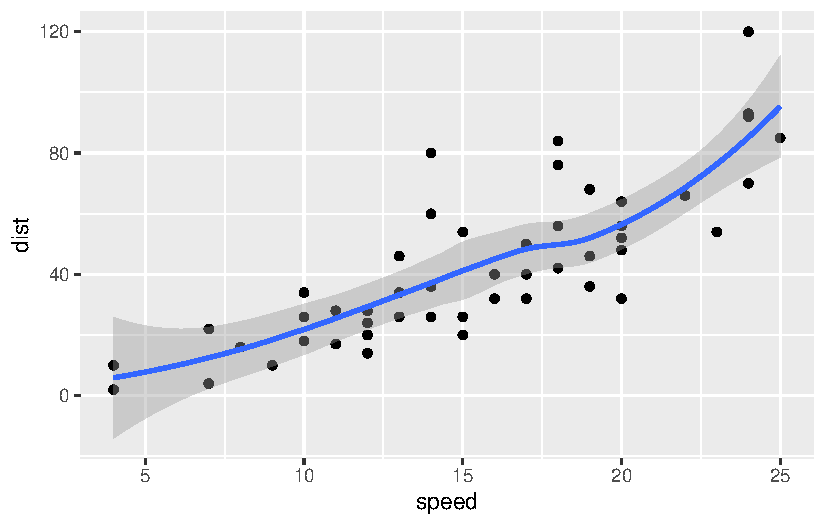
\includegraphics{class05_files/figure-pdf/unnamed-chunk-5-1.pdf}

}

\end{figure}

\begin{Shaded}
\begin{Highlighting}[]
\FunctionTok{ggplot}\NormalTok{(cars) }\SpecialCharTok{+}
  \FunctionTok{aes}\NormalTok{(}\AttributeTok{x =}\NormalTok{ speed, }\AttributeTok{y =}\NormalTok{ dist) }\SpecialCharTok{+}
  \FunctionTok{geom\_point}\NormalTok{() }\SpecialCharTok{+}
  \FunctionTok{geom\_smooth}\NormalTok{(}\AttributeTok{method =} \StringTok{"lm"}\NormalTok{, }\AttributeTok{se =} \ConstantTok{FALSE}\NormalTok{ )}
\end{Highlighting}
\end{Shaded}

\begin{verbatim}
`geom_smooth()` using formula = 'y ~ x'
\end{verbatim}

\begin{figure}[H]

{\centering 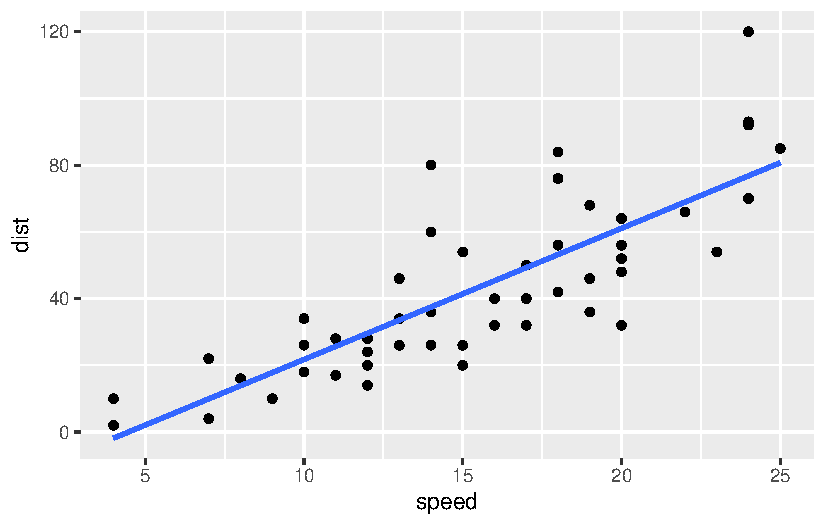
\includegraphics{class05_files/figure-pdf/unnamed-chunk-6-1.pdf}

}

\end{figure}

\begin{Shaded}
\begin{Highlighting}[]
\NormalTok{bp }\OtherTok{\textless{}{-}} \FunctionTok{ggplot}\NormalTok{(cars) }\SpecialCharTok{+}
  \FunctionTok{aes}\NormalTok{(}\AttributeTok{x =}\NormalTok{ speed, }\AttributeTok{y =}\NormalTok{ dist) }\SpecialCharTok{+}
  \FunctionTok{geom\_point}\NormalTok{() }\SpecialCharTok{+}
  \FunctionTok{geom\_smooth}\NormalTok{(}\AttributeTok{method =} \StringTok{"lm"}\NormalTok{, }\AttributeTok{se =} \ConstantTok{FALSE}\NormalTok{ )}\SpecialCharTok{+}
  \FunctionTok{labs}\NormalTok{(}\AttributeTok{title =} \StringTok{"Speed and stopping distance of cars"}\NormalTok{,}
      \AttributeTok{x =} \StringTok{"Speed (MPH)"}\NormalTok{, }
      \AttributeTok{y =} \StringTok{"Stopping distance (ft)"}\NormalTok{,}
      \AttributeTok{subtitle =} \StringTok{"MIT DUYYYYY"}\NormalTok{,}
      \AttributeTok{caption =} \StringTok{"Dataset = \textquotesingle{}cars\textquotesingle{}"}\NormalTok{) }\SpecialCharTok{+}
  \FunctionTok{theme\_bw}\NormalTok{()}

\NormalTok{bp}
\end{Highlighting}
\end{Shaded}

\begin{verbatim}
`geom_smooth()` using formula = 'y ~ x'
\end{verbatim}

\begin{figure}[H]

{\centering 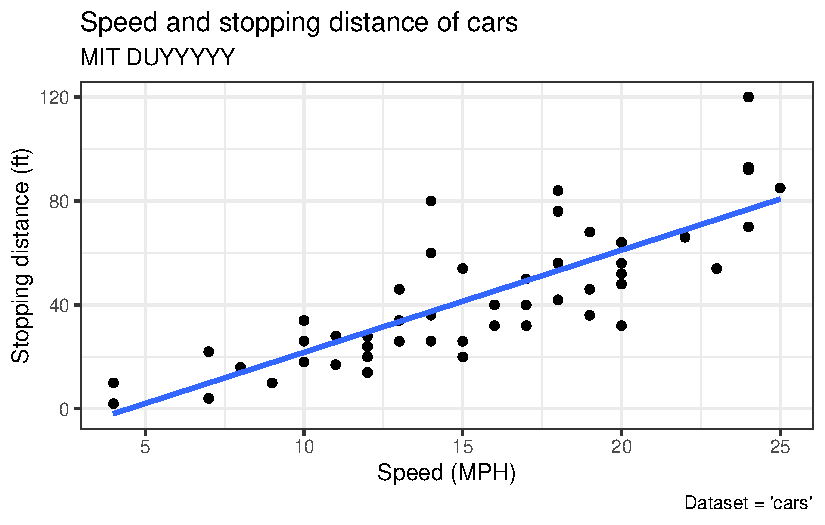
\includegraphics{class05_files/figure-pdf/unnamed-chunk-7-1.pdf}

}

\end{figure}

\hypertarget{a-more-complicated-scatter-plot}{%
\subsection{A more complicated scatter
plot}\label{a-more-complicated-scatter-plot}}

Here we make a plot of gene expression data:

\begin{Shaded}
\begin{Highlighting}[]
\NormalTok{url }\OtherTok{\textless{}{-}} \StringTok{"https://bioboot.github.io/bimm143\_S20/class{-}material/up\_down\_expression.txt"}
\NormalTok{genes }\OtherTok{\textless{}{-}} \FunctionTok{read.delim}\NormalTok{(url)}
\FunctionTok{head}\NormalTok{(genes)}
\end{Highlighting}
\end{Shaded}

\begin{verbatim}
        Gene Condition1 Condition2      State
1      A4GNT -3.6808610 -3.4401355 unchanging
2       AAAS  4.5479580  4.3864126 unchanging
3      AASDH  3.7190695  3.4787276 unchanging
4       AATF  5.0784720  5.0151916 unchanging
5       AATK  0.4711421  0.5598642 unchanging
6 AB015752.4 -3.6808610 -3.5921390 unchanging
\end{verbatim}

\begin{Shaded}
\begin{Highlighting}[]
\FunctionTok{nrow}\NormalTok{(genes)}
\end{Highlighting}
\end{Shaded}

\begin{verbatim}
[1] 5196
\end{verbatim}

\begin{Shaded}
\begin{Highlighting}[]
\FunctionTok{colnames}\NormalTok{(genes)}
\end{Highlighting}
\end{Shaded}

\begin{verbatim}
[1] "Gene"       "Condition1" "Condition2" "State"     
\end{verbatim}

\begin{Shaded}
\begin{Highlighting}[]
\FunctionTok{ncol}\NormalTok{(genes)}
\end{Highlighting}
\end{Shaded}

\begin{verbatim}
[1] 4
\end{verbatim}

\begin{Shaded}
\begin{Highlighting}[]
\FunctionTok{table}\NormalTok{(genes}\SpecialCharTok{$}\NormalTok{State)}
\end{Highlighting}
\end{Shaded}

\begin{verbatim}

      down unchanging         up 
        72       4997        127 
\end{verbatim}

\begin{Shaded}
\begin{Highlighting}[]
\FunctionTok{round}\NormalTok{(}\FunctionTok{table}\NormalTok{(genes}\SpecialCharTok{$}\NormalTok{State }\SpecialCharTok{==} \StringTok{\textquotesingle{}up\textquotesingle{}}\NormalTok{ )}\SpecialCharTok{/}\FunctionTok{nrow}\NormalTok{(genes) }\SpecialCharTok{*} \DecValTok{100}\NormalTok{, }\DecValTok{2}\NormalTok{ )}
\end{Highlighting}
\end{Shaded}

\begin{verbatim}

FALSE  TRUE 
97.56  2.44 
\end{verbatim}

\begin{Shaded}
\begin{Highlighting}[]
\NormalTok{n.gene }\OtherTok{\textless{}{-}} \FunctionTok{nrow}\NormalTok{(genes)}
\NormalTok{n.up }\OtherTok{\textless{}{-}} \FunctionTok{sum}\NormalTok{(genes}\SpecialCharTok{$}\NormalTok{State }\SpecialCharTok{==} \StringTok{\textquotesingle{}up\textquotesingle{}}\NormalTok{)}

\NormalTok{up.percent }\OtherTok{\textless{}{-}}\NormalTok{ n.up}\SpecialCharTok{/}\NormalTok{n.gene }\SpecialCharTok{*}\DecValTok{100}
\FunctionTok{round}\NormalTok{(up.percent, }\DecValTok{2}\NormalTok{)}
\end{Highlighting}
\end{Shaded}

\begin{verbatim}
[1] 2.44
\end{verbatim}

\begin{Shaded}
\begin{Highlighting}[]
\NormalTok{n }\OtherTok{\textless{}{-}} 
  \FunctionTok{ggplot}\NormalTok{(genes) }\SpecialCharTok{+}
  \FunctionTok{aes}\NormalTok{(}\AttributeTok{x =}\NormalTok{ Condition1, }\AttributeTok{y =}\NormalTok{ Condition2) }\SpecialCharTok{+}
  \FunctionTok{geom\_point}\NormalTok{()}

\NormalTok{n}
\end{Highlighting}
\end{Shaded}

\begin{figure}[H]

{\centering 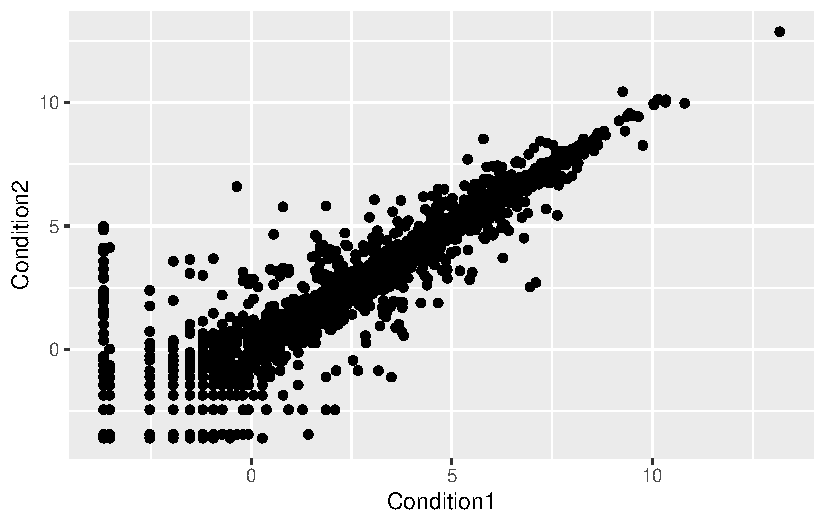
\includegraphics{class05_files/figure-pdf/unnamed-chunk-11-1.pdf}

}

\end{figure}

\begin{Shaded}
\begin{Highlighting}[]
\NormalTok{gene\_plot }\OtherTok{\textless{}{-}}\NormalTok{ n }\SpecialCharTok{+} \FunctionTok{aes}\NormalTok{(}\AttributeTok{col =}\NormalTok{ State)}

\NormalTok{gene\_plot}
\end{Highlighting}
\end{Shaded}

\begin{figure}[H]

{\centering 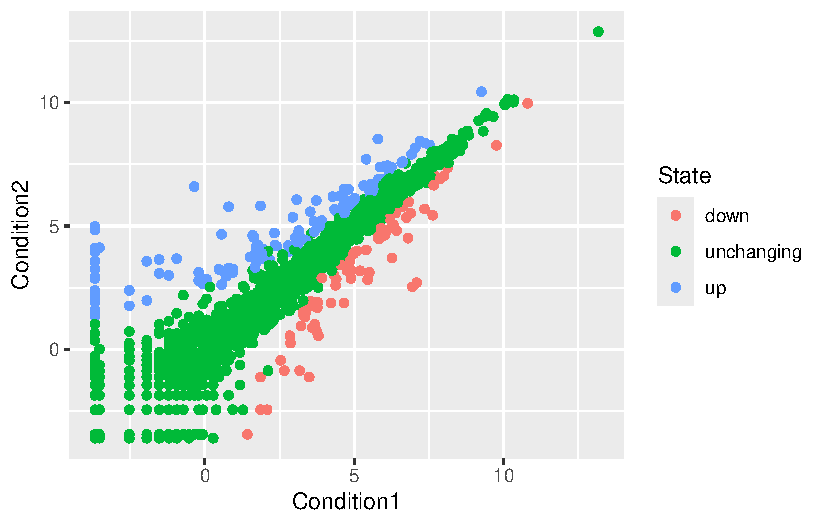
\includegraphics{class05_files/figure-pdf/unnamed-chunk-12-1.pdf}

}

\end{figure}

\begin{Shaded}
\begin{Highlighting}[]
\NormalTok{gene\_plot }\SpecialCharTok{+} \FunctionTok{scale\_color\_manual}\NormalTok{(}\AttributeTok{values =} \FunctionTok{c}\NormalTok{(}\StringTok{"blue"}\NormalTok{, }\StringTok{"gray"}\NormalTok{, }\StringTok{"red"}\NormalTok{)) }\SpecialCharTok{+}
  \FunctionTok{labs}\NormalTok{(}\AttributeTok{x =} \StringTok{"Control(no drug)"}\NormalTok{, }\AttributeTok{y =} \StringTok{"Drug Treatment"}\NormalTok{, }\AttributeTok{title =} \StringTok{"Gene Expression Changing Upon Drug Treatment"}\NormalTok{)}
\end{Highlighting}
\end{Shaded}

\begin{figure}[H]

{\centering 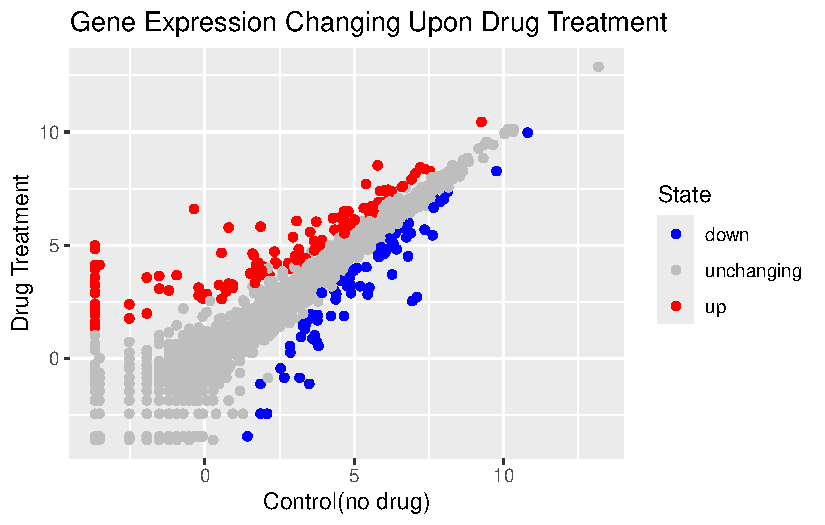
\includegraphics{class05_files/figure-pdf/unnamed-chunk-13-1.pdf}

}

\end{figure}

\hypertarget{exploring-the-gapminder-dataset}{%
\subsection{Exploring the gapminder
dataset}\label{exploring-the-gapminder-dataset}}

\begin{Shaded}
\begin{Highlighting}[]
\FunctionTok{library}\NormalTok{(gapminder)}
\CommentTok{\# File location online}
\NormalTok{url }\OtherTok{\textless{}{-}} \StringTok{"https://raw.githubusercontent.com/jennybc/gapminder/master/inst/extdata/gapminder.tsv"}
\NormalTok{gapminder }\OtherTok{\textless{}{-}} \FunctionTok{read.delim}\NormalTok{(url)}
\end{Highlighting}
\end{Shaded}

\begin{Shaded}
\begin{Highlighting}[]
\FunctionTok{head}\NormalTok{(gapminder)}
\end{Highlighting}
\end{Shaded}

\begin{verbatim}
      country continent year lifeExp      pop gdpPercap
1 Afghanistan      Asia 1952  28.801  8425333  779.4453
2 Afghanistan      Asia 1957  30.332  9240934  820.8530
3 Afghanistan      Asia 1962  31.997 10267083  853.1007
4 Afghanistan      Asia 1967  34.020 11537966  836.1971
5 Afghanistan      Asia 1972  36.088 13079460  739.9811
6 Afghanistan      Asia 1977  38.438 14880372  786.1134
\end{verbatim}

\begin{quote}
Q. How many continent are there? Use function \texttt{unique()}
\end{quote}

\begin{Shaded}
\begin{Highlighting}[]
\NormalTok{num }\OtherTok{\textless{}{-}} \FunctionTok{unique}\NormalTok{(gapminder}\SpecialCharTok{$}\NormalTok{continent)}
\FunctionTok{length}\NormalTok{(num)}
\end{Highlighting}
\end{Shaded}

\begin{verbatim}
[1] 5
\end{verbatim}

\begin{quote}
Q. How many countries are there?
\end{quote}

\begin{Shaded}
\begin{Highlighting}[]
\NormalTok{num }\OtherTok{\textless{}{-}} \FunctionTok{unique}\NormalTok{(gapminder}\SpecialCharTok{$}\NormalTok{country)}
\FunctionTok{length}\NormalTok{(num)}
\end{Highlighting}
\end{Shaded}

\begin{verbatim}
[1] 142
\end{verbatim}

\begin{Shaded}
\begin{Highlighting}[]
\FunctionTok{library}\NormalTok{(dplyr)}
\end{Highlighting}
\end{Shaded}

\begin{verbatim}

Attaching package: 'dplyr'
\end{verbatim}

\begin{verbatim}
The following objects are masked from 'package:stats':

    filter, lag
\end{verbatim}

\begin{verbatim}
The following objects are masked from 'package:base':

    intersect, setdiff, setequal, union
\end{verbatim}

\begin{Shaded}
\begin{Highlighting}[]
\NormalTok{gapminder\_2007 }\OtherTok{\textless{}{-}}\NormalTok{ gapminder }\SpecialCharTok{\%\textgreater{}\%} \FunctionTok{filter}\NormalTok{(year}\SpecialCharTok{==}\DecValTok{2007}\NormalTok{)}
\FunctionTok{head}\NormalTok{(gapminder\_2007)}
\end{Highlighting}
\end{Shaded}

\begin{verbatim}
      country continent year lifeExp      pop  gdpPercap
1 Afghanistan      Asia 2007  43.828 31889923   974.5803
2     Albania    Europe 2007  76.423  3600523  5937.0295
3     Algeria    Africa 2007  72.301 33333216  6223.3675
4      Angola    Africa 2007  42.731 12420476  4797.2313
5   Argentina  Americas 2007  75.320 40301927 12779.3796
6   Australia   Oceania 2007  81.235 20434176 34435.3674
\end{verbatim}

\begin{Shaded}
\begin{Highlighting}[]
\FunctionTok{library}\NormalTok{(ggplot2)}
\FunctionTok{ggplot}\NormalTok{(gapminder\_2007) }\SpecialCharTok{+} 
  \FunctionTok{aes}\NormalTok{(}\AttributeTok{x =}\NormalTok{ gdpPercap, }\AttributeTok{y =}\NormalTok{ lifeExp) }\SpecialCharTok{+}
  \FunctionTok{geom\_point}\NormalTok{(}\AttributeTok{alpha=}\FloatTok{0.5}\NormalTok{)}
\end{Highlighting}
\end{Shaded}

\begin{figure}[H]

{\centering 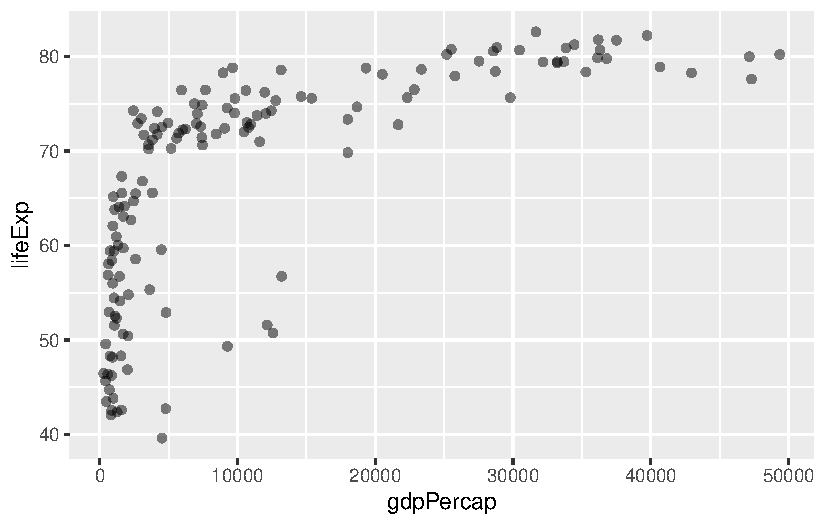
\includegraphics{class05_files/figure-pdf/unnamed-chunk-19-1.pdf}

}

\end{figure}

\begin{Shaded}
\begin{Highlighting}[]
\FunctionTok{ggplot}\NormalTok{(gapminder\_2007) }\SpecialCharTok{+} 
  \FunctionTok{aes}\NormalTok{(}\AttributeTok{x =}\NormalTok{ gdpPercap, }\AttributeTok{y =}\NormalTok{ lifeExp, }\AttributeTok{color =}\NormalTok{ continent, }\AttributeTok{size =}\NormalTok{ pop) }\SpecialCharTok{+}
  \FunctionTok{geom\_point}\NormalTok{(}\AttributeTok{alpha=}\FloatTok{0.5}\NormalTok{)}
\end{Highlighting}
\end{Shaded}

\begin{figure}[H]

{\centering 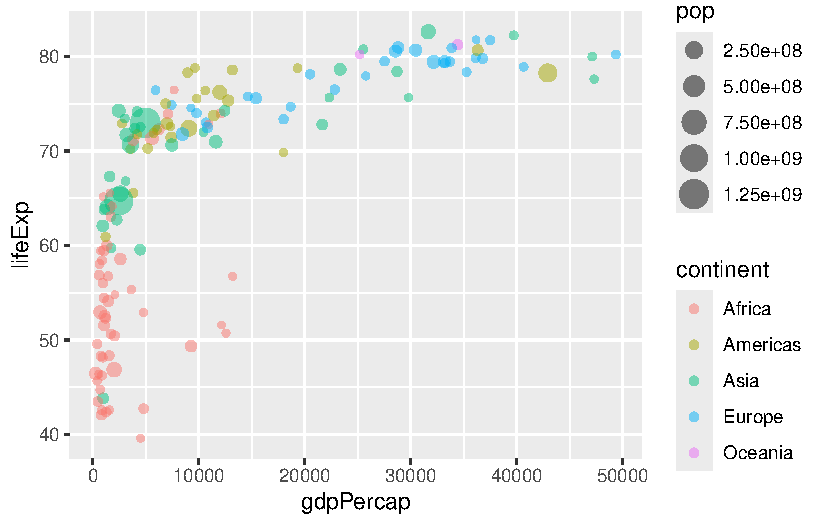
\includegraphics{class05_files/figure-pdf/unnamed-chunk-20-1.pdf}

}

\end{figure}

\begin{Shaded}
\begin{Highlighting}[]
\FunctionTok{ggplot}\NormalTok{(gapminder\_2007) }\SpecialCharTok{+} 
  \FunctionTok{aes}\NormalTok{(}\AttributeTok{x =}\NormalTok{ gdpPercap, }\AttributeTok{y =}\NormalTok{ lifeExp, }\AttributeTok{color =}\NormalTok{ pop) }\SpecialCharTok{+}
  \FunctionTok{geom\_point}\NormalTok{(}\AttributeTok{alpha=}\FloatTok{0.7}\NormalTok{)}
\end{Highlighting}
\end{Shaded}

\begin{figure}[H]

{\centering 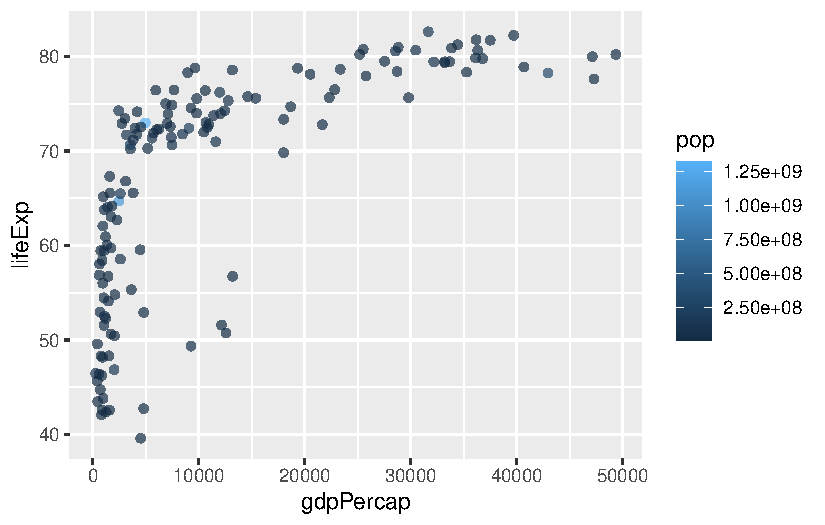
\includegraphics{class05_files/figure-pdf/unnamed-chunk-21-1.pdf}

}

\end{figure}

\begin{quote}
Q. How to reflect the real population on the size of the points
\end{quote}

\begin{Shaded}
\begin{Highlighting}[]
\FunctionTok{ggplot}\NormalTok{(gapminder\_2007) }\SpecialCharTok{+} 
  \FunctionTok{geom\_point}\NormalTok{(}\FunctionTok{aes}\NormalTok{(}\AttributeTok{x =}\NormalTok{ gdpPercap, }\AttributeTok{y =}\NormalTok{ lifeExp,}
                 \AttributeTok{size =}\NormalTok{ pop), }\AttributeTok{alpha=}\FloatTok{0.5}\NormalTok{) }\SpecialCharTok{+} 
  \FunctionTok{scale\_size\_area}\NormalTok{(}\AttributeTok{max\_size =} \DecValTok{10}\NormalTok{)}
\end{Highlighting}
\end{Shaded}

\begin{figure}[H]

{\centering 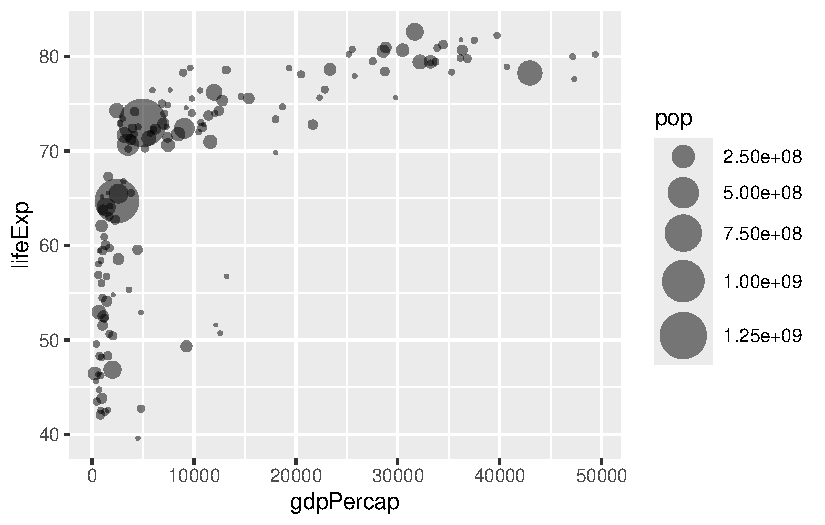
\includegraphics{class05_files/figure-pdf/unnamed-chunk-22-1.pdf}

}

\end{figure}

\begin{quote}
Q. Can you adapt the code you have learned thus far to reproduce our
gapminder scatter plot for the year 1957? What do you notice about this
plot is it easy to compare with the one for 2007?
\end{quote}

\begin{Shaded}
\begin{Highlighting}[]
\NormalTok{gapminder\_1957 }\OtherTok{\textless{}{-}}\NormalTok{ gapminder }\SpecialCharTok{\%\textgreater{}\%} \FunctionTok{filter}\NormalTok{(year }\SpecialCharTok{==} \DecValTok{2007} \SpecialCharTok{|}\NormalTok{ year}\SpecialCharTok{==}\DecValTok{1957}\NormalTok{)}
\FunctionTok{ggplot}\NormalTok{(gapminder\_1957) }\SpecialCharTok{+}
  \FunctionTok{aes}\NormalTok{(}\AttributeTok{x =}\NormalTok{ gdpPercap, }\AttributeTok{y =}\NormalTok{ lifeExp, }\AttributeTok{color =}\NormalTok{ continent, }\AttributeTok{size =}\NormalTok{ pop) }\SpecialCharTok{+}
  \FunctionTok{geom\_point}\NormalTok{() }\SpecialCharTok{+} 
  \FunctionTok{scale\_size\_area}\NormalTok{(}\AttributeTok{max\_size =} \DecValTok{10}\NormalTok{) }\SpecialCharTok{+}
  \FunctionTok{facet\_wrap}\NormalTok{(}\SpecialCharTok{\textasciitilde{}}\NormalTok{year)}
\end{Highlighting}
\end{Shaded}

\begin{figure}[H]

{\centering 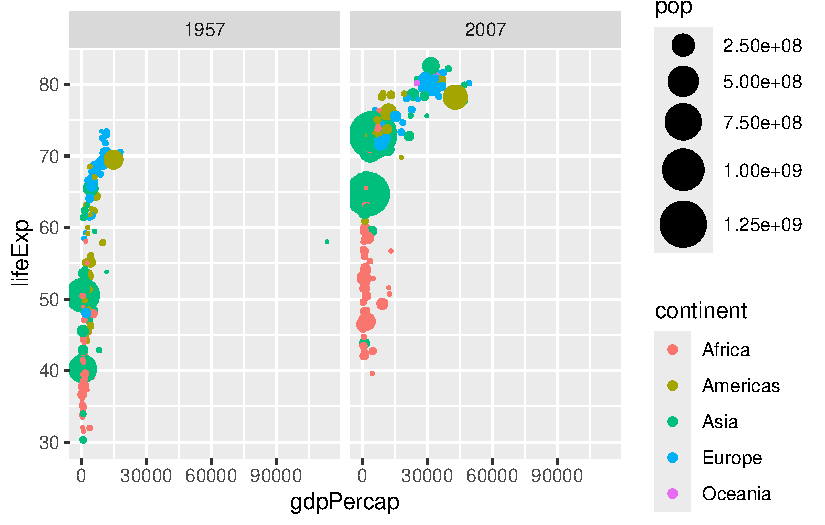
\includegraphics{class05_files/figure-pdf/unnamed-chunk-23-1.pdf}

}

\end{figure}

\hypertarget{animation}{%
\subsection{Animation}\label{animation}}

\begin{Shaded}
\begin{Highlighting}[]
\FunctionTok{library}\NormalTok{(gapminder)}
\FunctionTok{library}\NormalTok{(gganimate)}
\CommentTok{\# Setup nice regular ggplot of the gapminder data}
\FunctionTok{ggplot}\NormalTok{(gapminder, }\FunctionTok{aes}\NormalTok{(gdpPercap, lifeExp, }\AttributeTok{size =}\NormalTok{ pop, }\AttributeTok{colour =}\NormalTok{ country)) }\SpecialCharTok{+}
  \FunctionTok{geom\_point}\NormalTok{(}\AttributeTok{alpha =} \FloatTok{0.7}\NormalTok{, }\AttributeTok{show.legend =} \ConstantTok{FALSE}\NormalTok{) }\SpecialCharTok{+}
  \FunctionTok{scale\_colour\_manual}\NormalTok{(}\AttributeTok{values =}\NormalTok{ country\_colors) }\SpecialCharTok{+}
  \FunctionTok{scale\_size}\NormalTok{(}\AttributeTok{range =} \FunctionTok{c}\NormalTok{(}\DecValTok{2}\NormalTok{, }\DecValTok{12}\NormalTok{)) }\SpecialCharTok{+}
  \FunctionTok{scale\_x\_log10}\NormalTok{() }\SpecialCharTok{+}
  \CommentTok{\# Facet by continent}
  \FunctionTok{facet\_wrap}\NormalTok{(}\SpecialCharTok{\textasciitilde{}}\NormalTok{continent) }\SpecialCharTok{+}
  \CommentTok{\# Here comes the gganimate specific bits}
  \FunctionTok{labs}\NormalTok{(}\AttributeTok{title =} \StringTok{\textquotesingle{}Year: \{frame\_time\}\textquotesingle{}}\NormalTok{, }\AttributeTok{x =} \StringTok{\textquotesingle{}GDP per capita\textquotesingle{}}\NormalTok{, }\AttributeTok{y =} \StringTok{\textquotesingle{}life expectancy\textquotesingle{}}\NormalTok{) }\SpecialCharTok{+}
  \FunctionTok{transition\_time}\NormalTok{(year) }\SpecialCharTok{+}
  \FunctionTok{shadow\_wake}\NormalTok{(}\AttributeTok{wake\_length =} \FloatTok{0.1}\NormalTok{, }\AttributeTok{alpha =} \ConstantTok{FALSE}\NormalTok{)}
\end{Highlighting}
\end{Shaded}

\begin{verbatim}
Warning in formals(fun): argument is not a function
\end{verbatim}

\begin{figure}[H]

{\centering 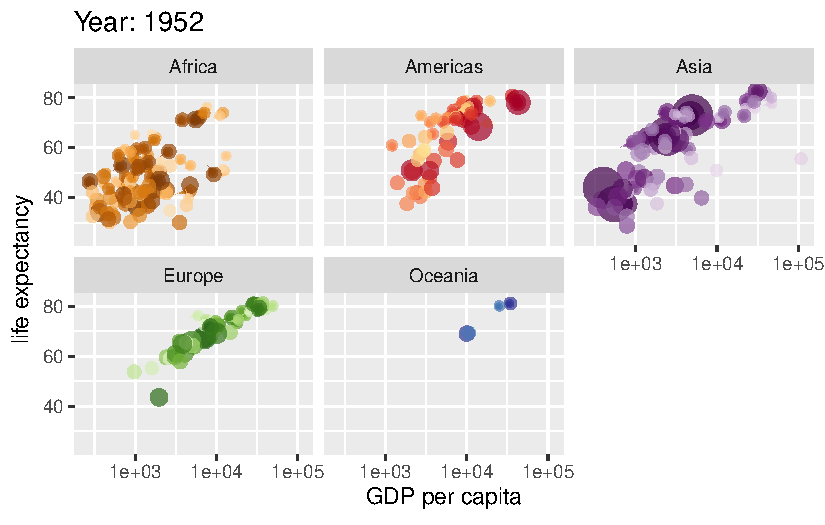
\includegraphics{class05_files/figure-pdf/unnamed-chunk-24-1.pdf}

}

\end{figure}

\begin{figure}[H]

{\centering 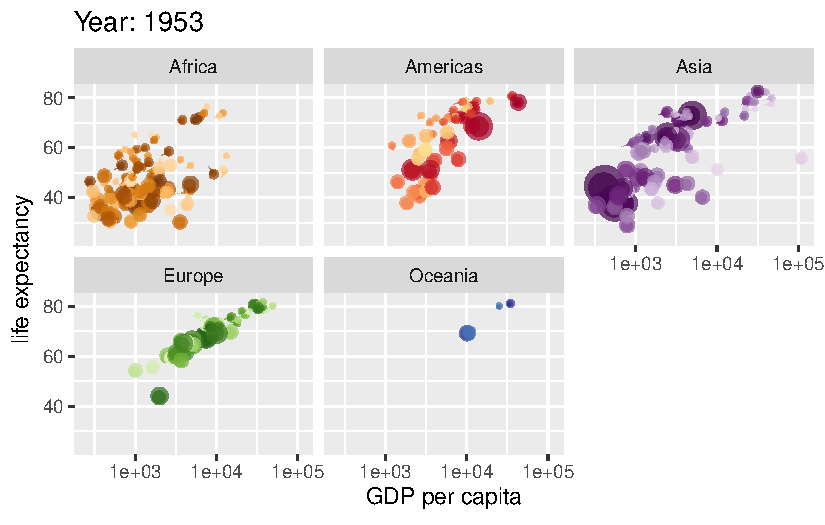
\includegraphics{class05_files/figure-pdf/unnamed-chunk-24-2.pdf}

}

\end{figure}

\begin{figure}[H]

{\centering 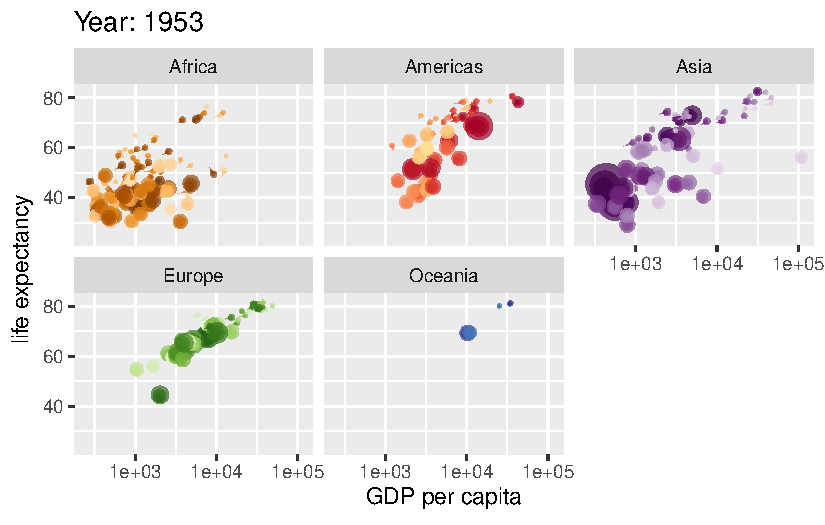
\includegraphics{class05_files/figure-pdf/unnamed-chunk-24-3.pdf}

}

\end{figure}

\begin{figure}[H]

{\centering 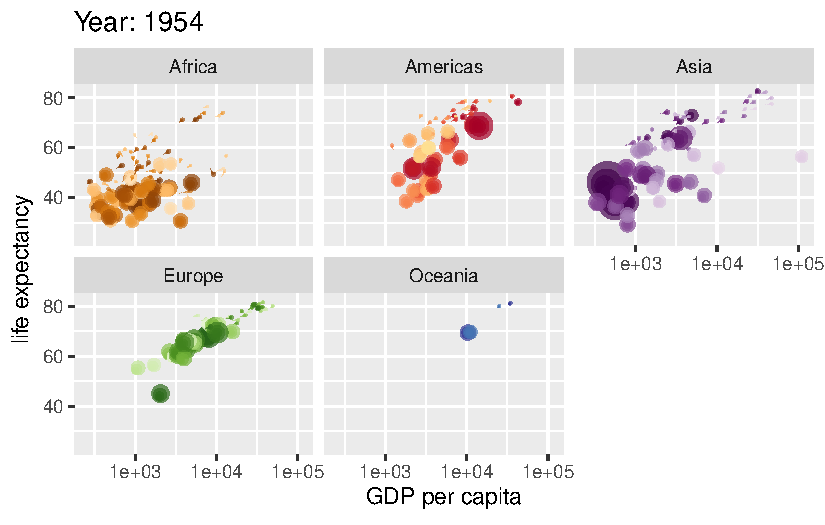
\includegraphics{class05_files/figure-pdf/unnamed-chunk-24-4.pdf}

}

\end{figure}

\begin{figure}[H]

{\centering 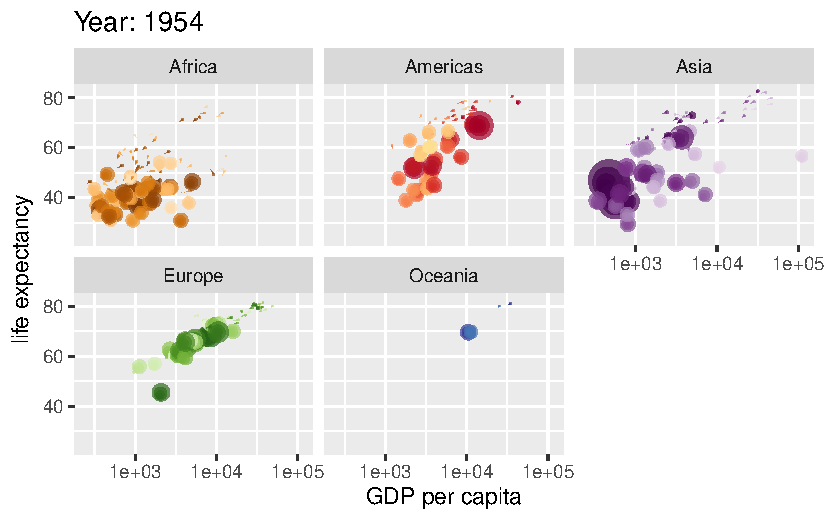
\includegraphics{class05_files/figure-pdf/unnamed-chunk-24-5.pdf}

}

\end{figure}

\begin{figure}[H]

{\centering 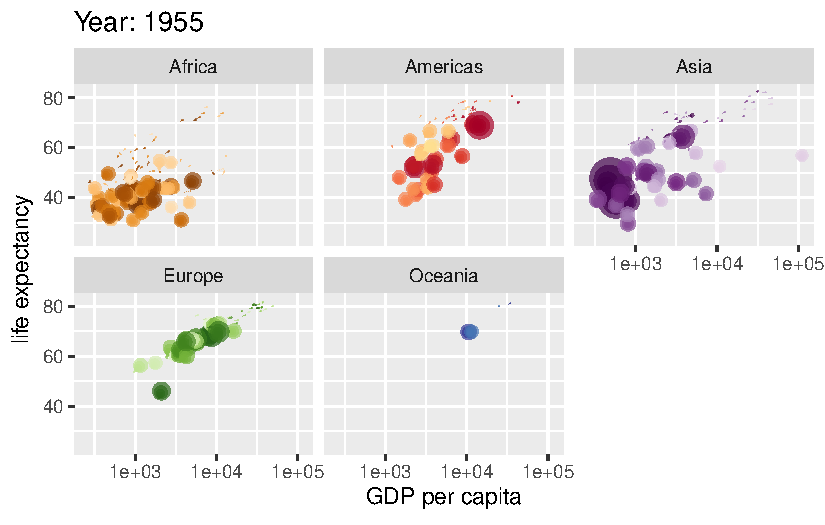
\includegraphics{class05_files/figure-pdf/unnamed-chunk-24-6.pdf}

}

\end{figure}

\begin{figure}[H]

{\centering 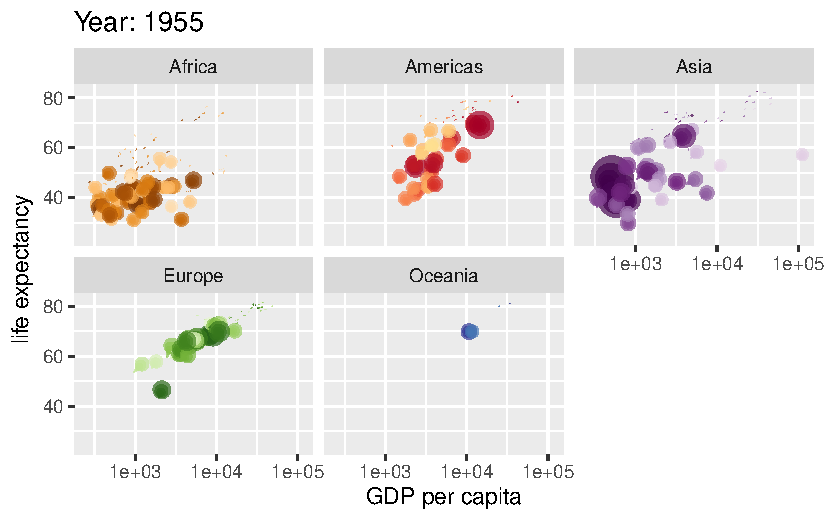
\includegraphics{class05_files/figure-pdf/unnamed-chunk-24-7.pdf}

}

\end{figure}

\begin{figure}[H]

{\centering 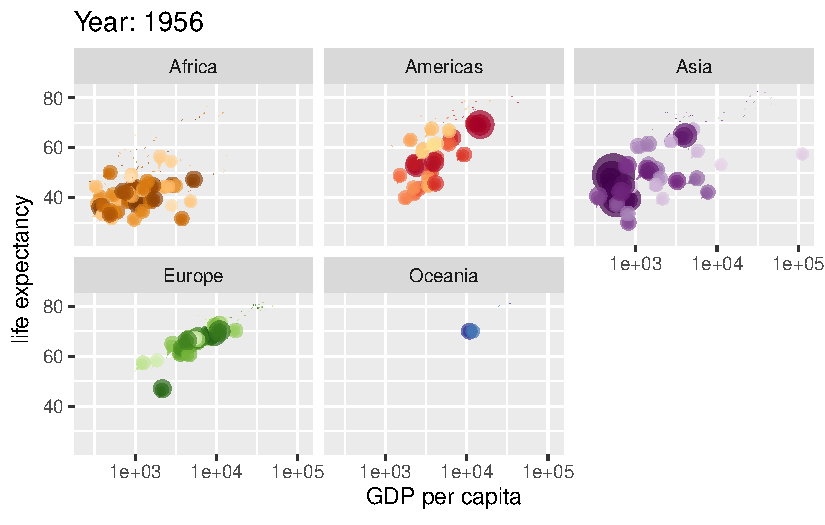
\includegraphics{class05_files/figure-pdf/unnamed-chunk-24-8.pdf}

}

\end{figure}

\begin{figure}[H]

{\centering 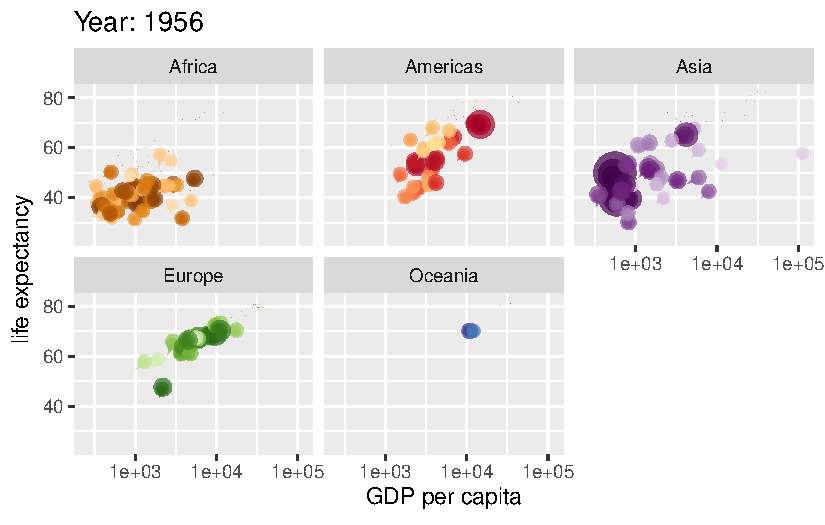
\includegraphics{class05_files/figure-pdf/unnamed-chunk-24-9.pdf}

}

\end{figure}

\begin{figure}[H]

{\centering 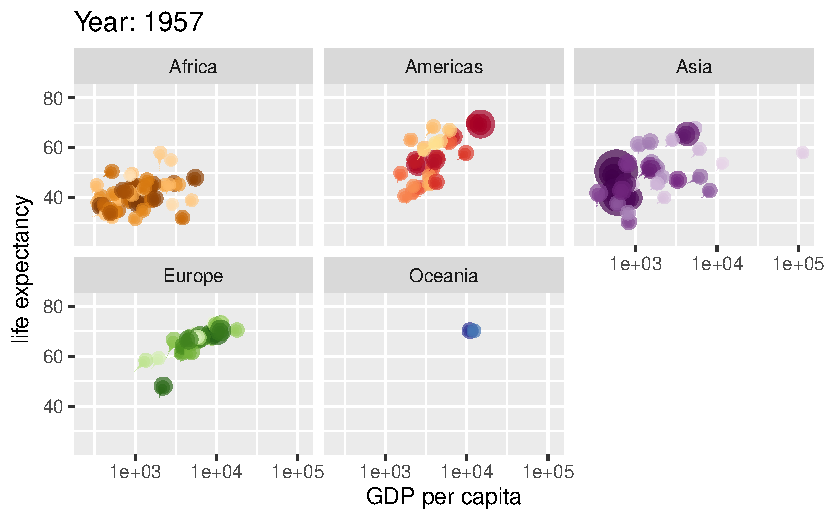
\includegraphics{class05_files/figure-pdf/unnamed-chunk-24-10.pdf}

}

\end{figure}

\begin{figure}[H]

{\centering 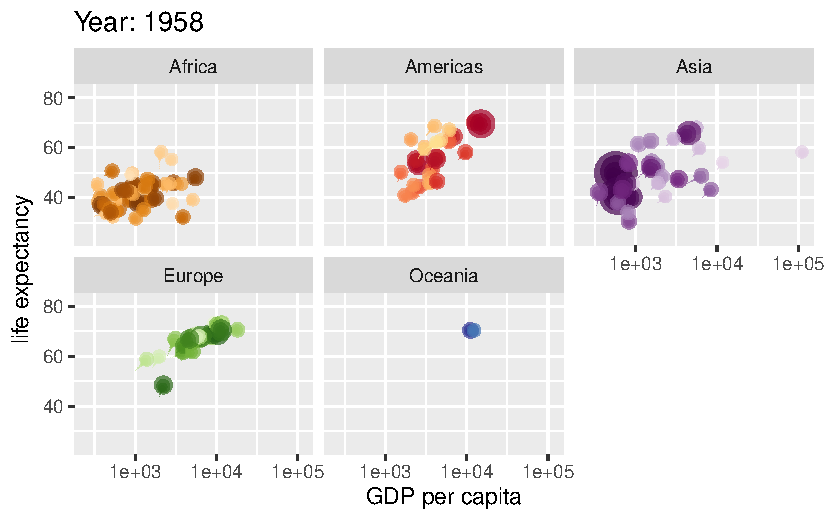
\includegraphics{class05_files/figure-pdf/unnamed-chunk-24-11.pdf}

}

\end{figure}

\begin{figure}[H]

{\centering 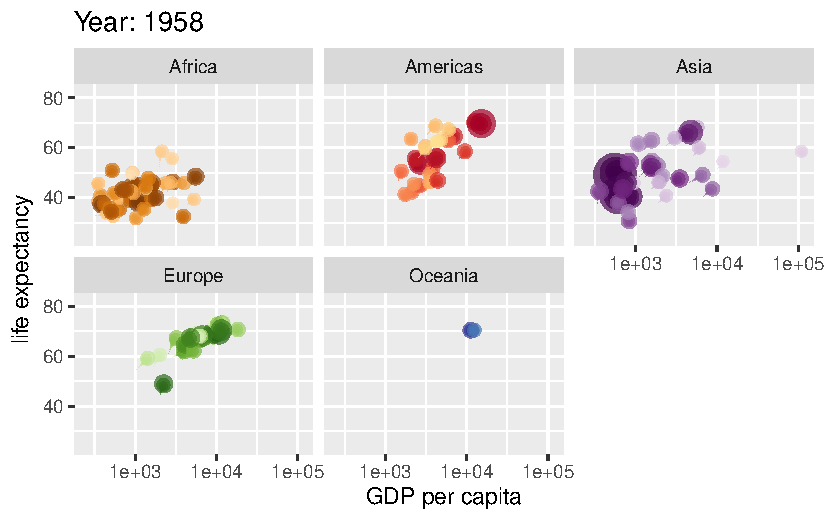
\includegraphics{class05_files/figure-pdf/unnamed-chunk-24-12.pdf}

}

\end{figure}

\begin{figure}[H]

{\centering 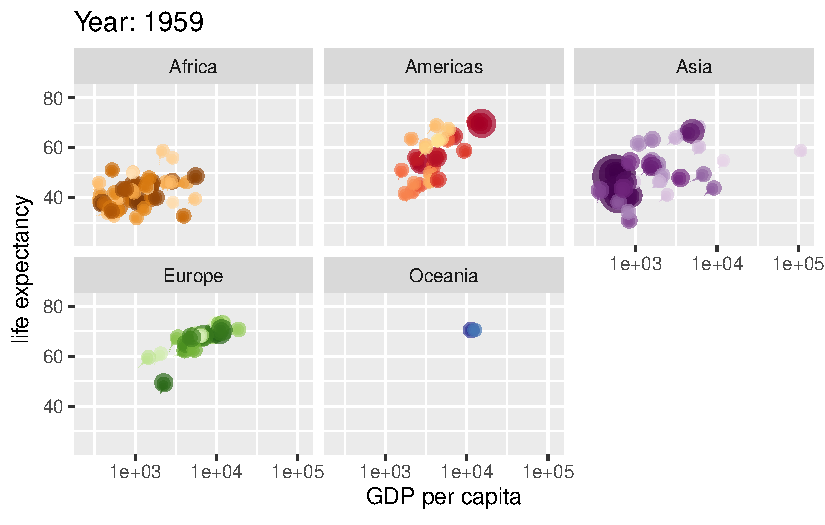
\includegraphics{class05_files/figure-pdf/unnamed-chunk-24-13.pdf}

}

\end{figure}

\begin{figure}[H]

{\centering 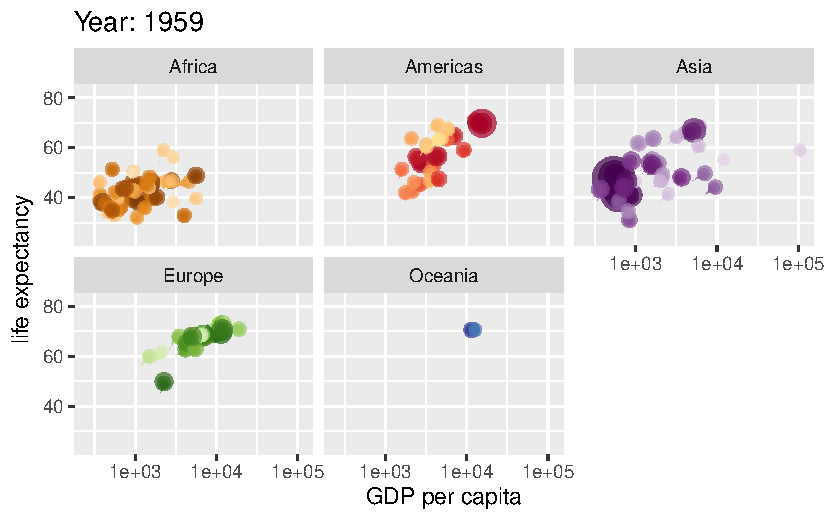
\includegraphics{class05_files/figure-pdf/unnamed-chunk-24-14.pdf}

}

\end{figure}

\begin{figure}[H]

{\centering 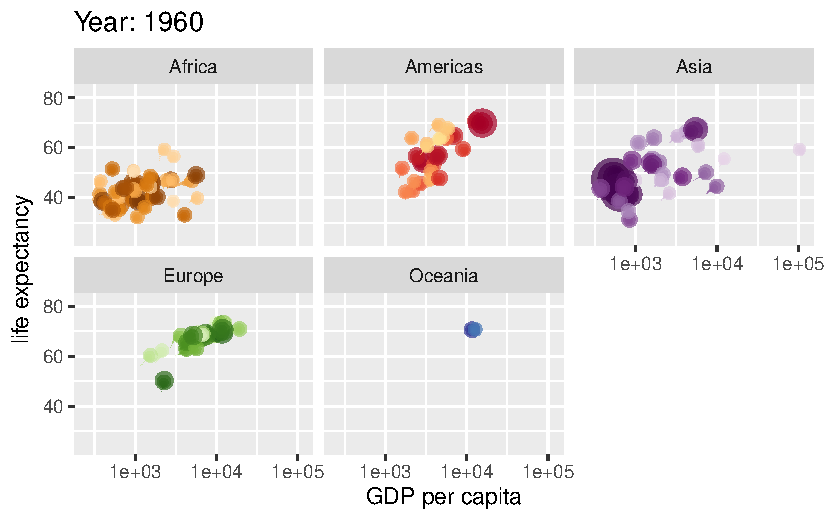
\includegraphics{class05_files/figure-pdf/unnamed-chunk-24-15.pdf}

}

\end{figure}

\begin{figure}[H]

{\centering 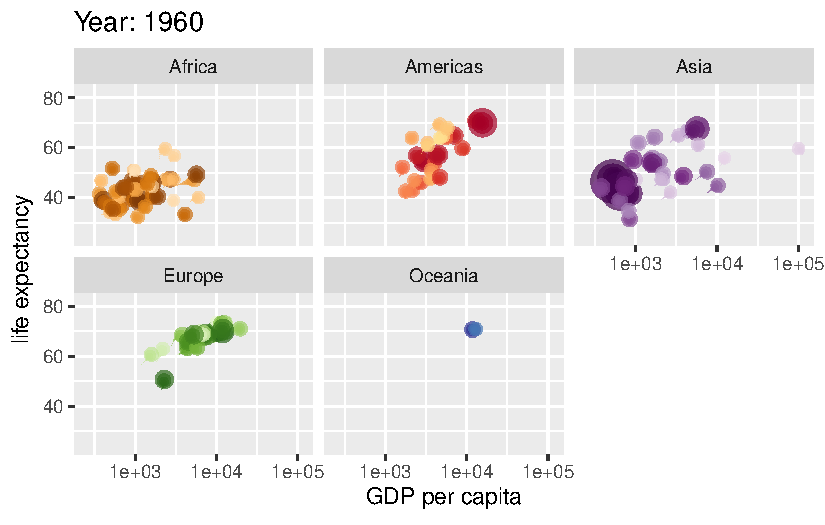
\includegraphics{class05_files/figure-pdf/unnamed-chunk-24-16.pdf}

}

\end{figure}

\begin{figure}[H]

{\centering 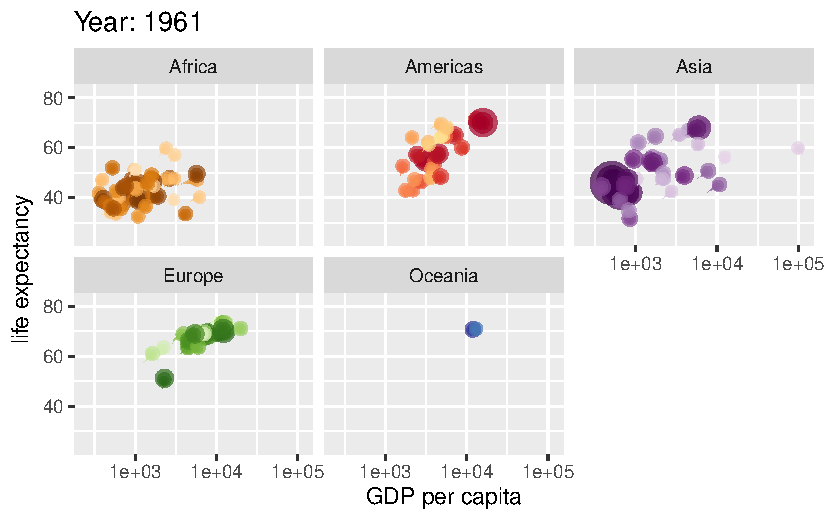
\includegraphics{class05_files/figure-pdf/unnamed-chunk-24-17.pdf}

}

\end{figure}

\begin{figure}[H]

{\centering 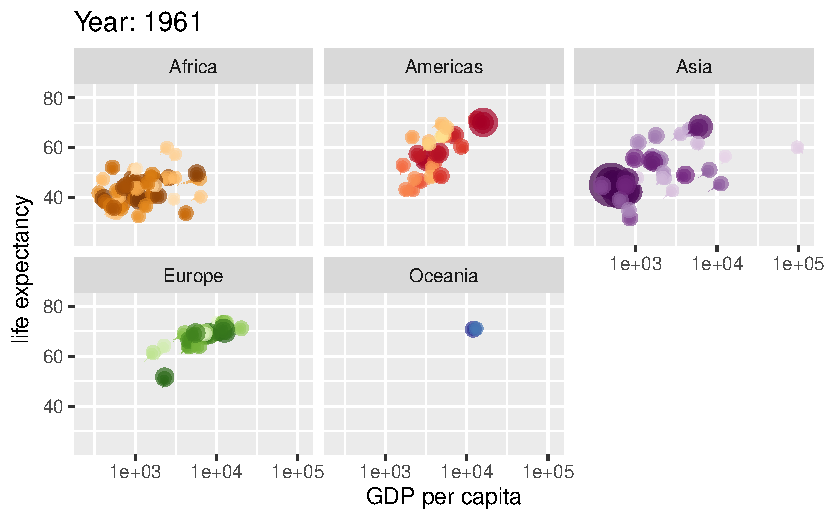
\includegraphics{class05_files/figure-pdf/unnamed-chunk-24-18.pdf}

}

\end{figure}

\begin{figure}[H]

{\centering 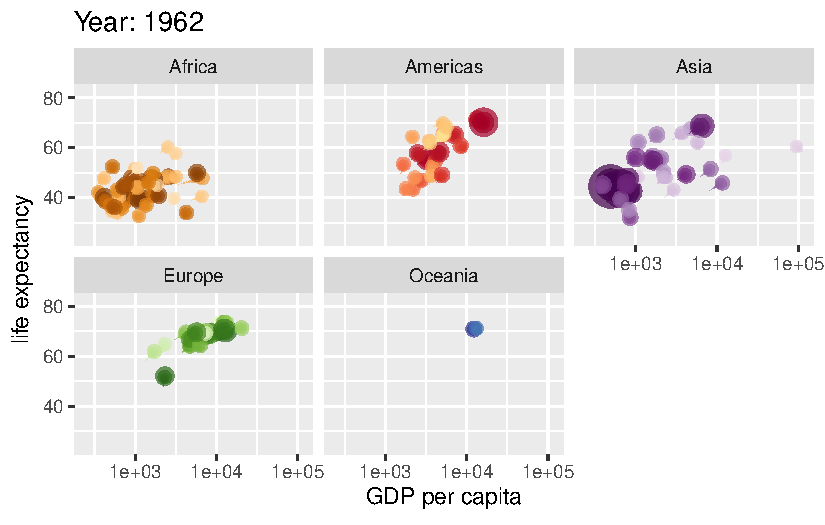
\includegraphics{class05_files/figure-pdf/unnamed-chunk-24-19.pdf}

}

\end{figure}

\begin{figure}[H]

{\centering 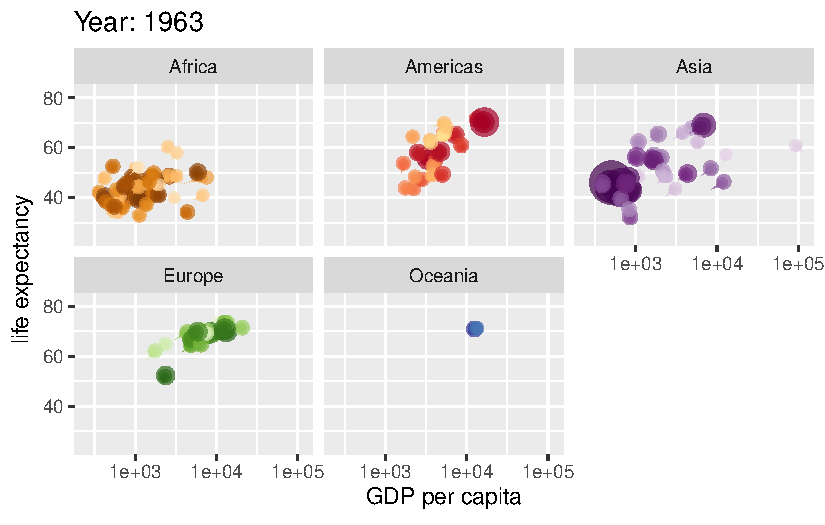
\includegraphics{class05_files/figure-pdf/unnamed-chunk-24-20.pdf}

}

\end{figure}

\begin{figure}[H]

{\centering 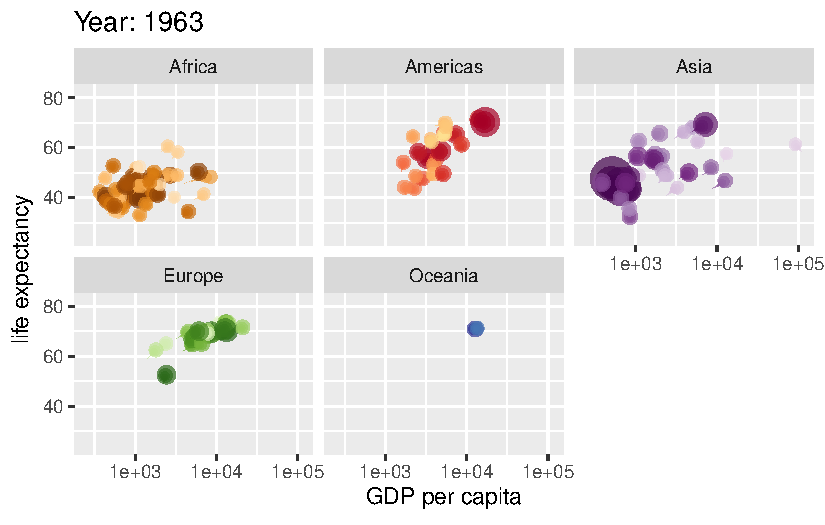
\includegraphics{class05_files/figure-pdf/unnamed-chunk-24-21.pdf}

}

\end{figure}

\begin{figure}[H]

{\centering 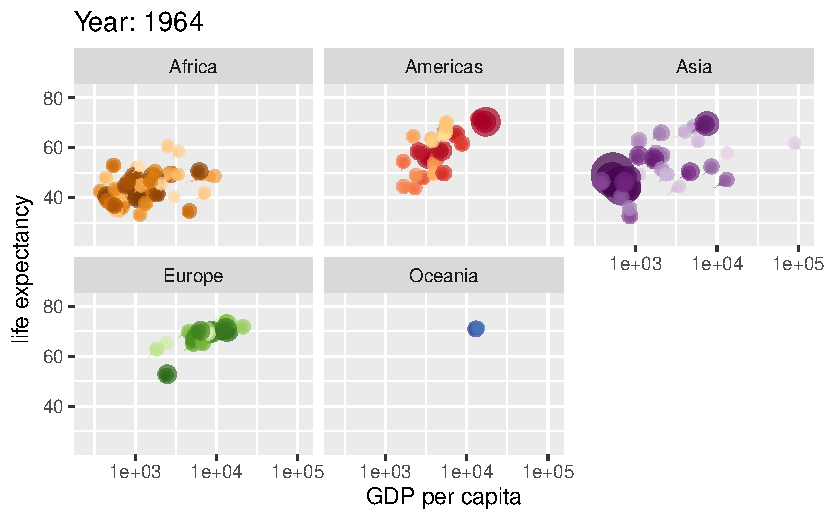
\includegraphics{class05_files/figure-pdf/unnamed-chunk-24-22.pdf}

}

\end{figure}

\begin{figure}[H]

{\centering 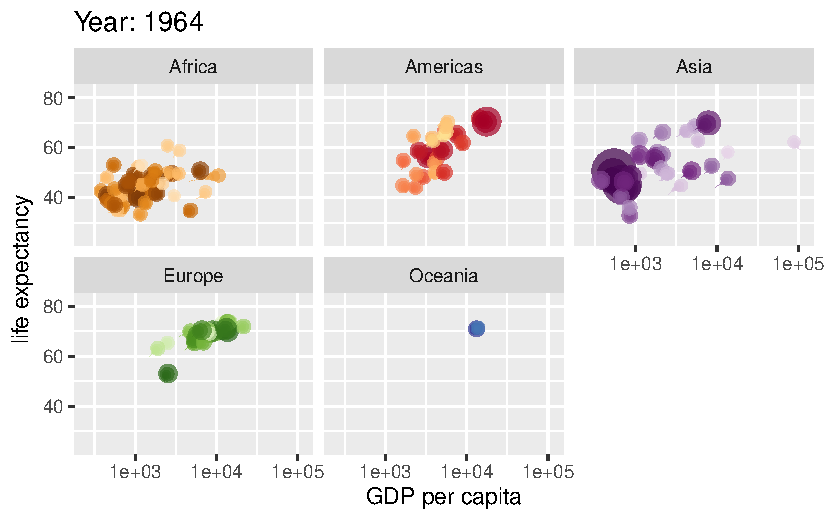
\includegraphics{class05_files/figure-pdf/unnamed-chunk-24-23.pdf}

}

\end{figure}

\begin{figure}[H]

{\centering 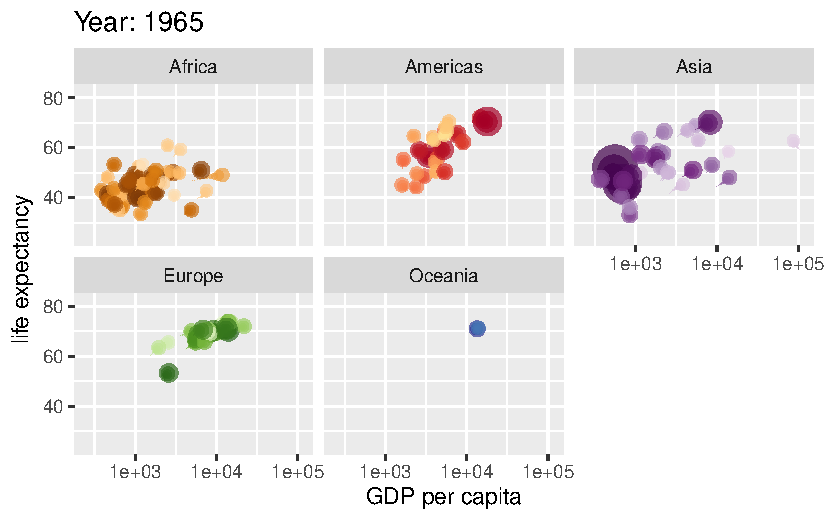
\includegraphics{class05_files/figure-pdf/unnamed-chunk-24-24.pdf}

}

\end{figure}

\begin{figure}[H]

{\centering 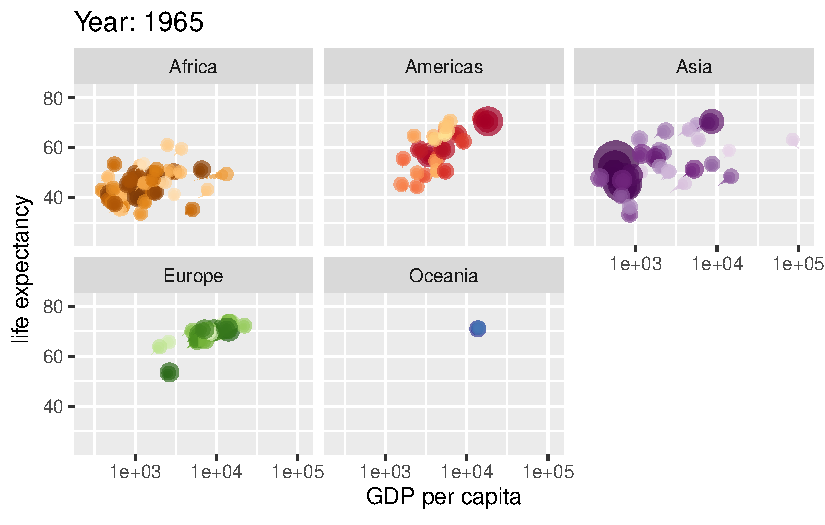
\includegraphics{class05_files/figure-pdf/unnamed-chunk-24-25.pdf}

}

\end{figure}

\begin{figure}[H]

{\centering 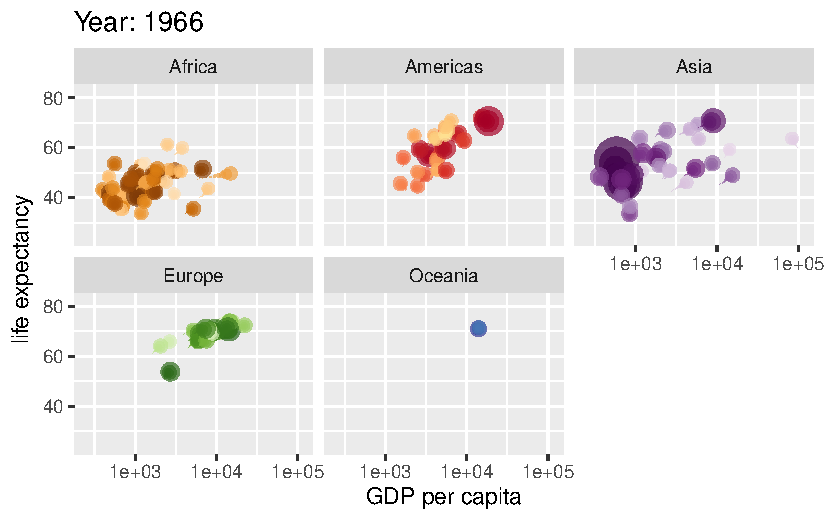
\includegraphics{class05_files/figure-pdf/unnamed-chunk-24-26.pdf}

}

\end{figure}

\begin{figure}[H]

{\centering 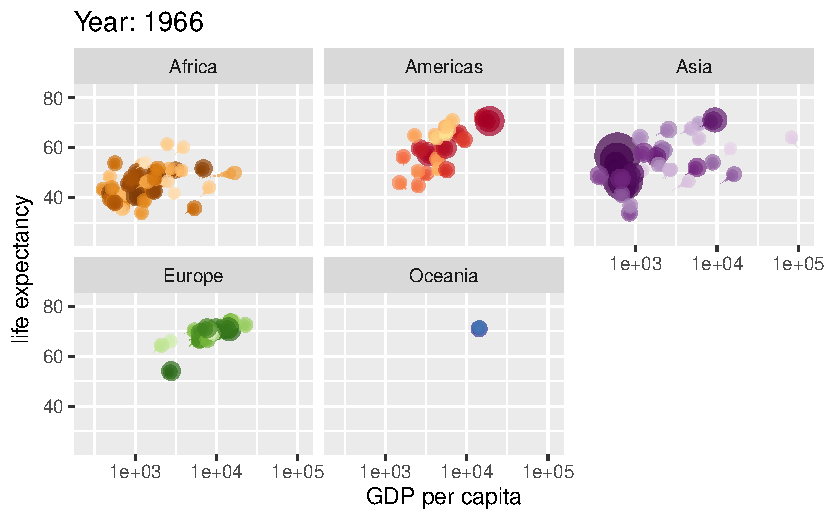
\includegraphics{class05_files/figure-pdf/unnamed-chunk-24-27.pdf}

}

\end{figure}

\begin{figure}[H]

{\centering 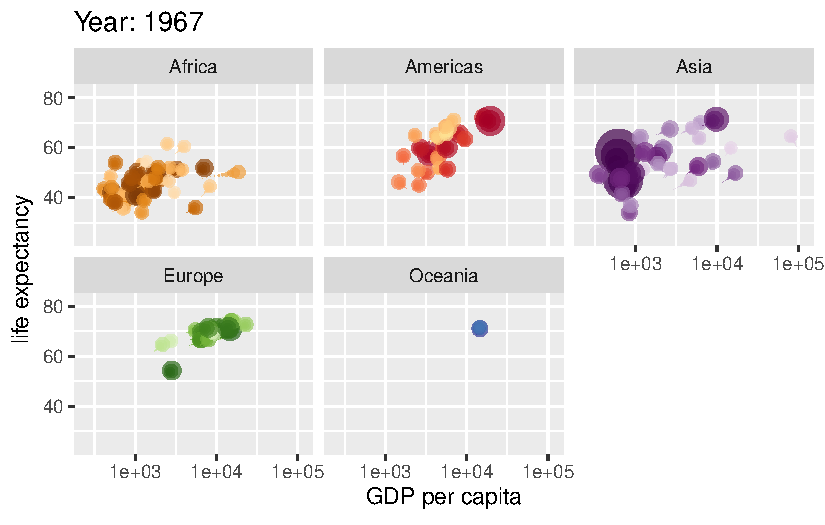
\includegraphics{class05_files/figure-pdf/unnamed-chunk-24-28.pdf}

}

\end{figure}

\begin{figure}[H]

{\centering 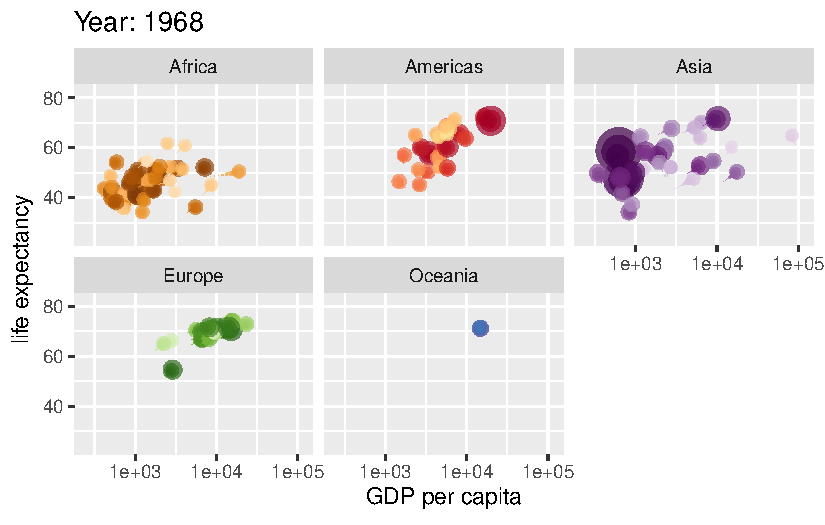
\includegraphics{class05_files/figure-pdf/unnamed-chunk-24-29.pdf}

}

\end{figure}

\begin{figure}[H]

{\centering 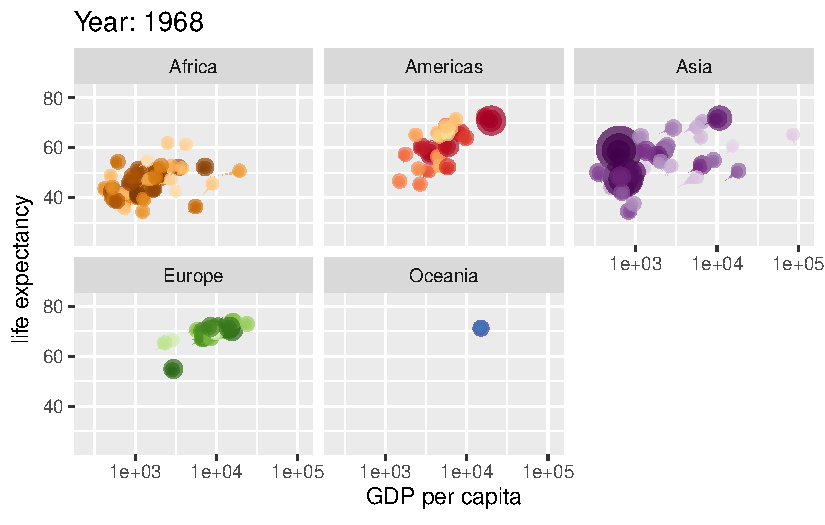
\includegraphics{class05_files/figure-pdf/unnamed-chunk-24-30.pdf}

}

\end{figure}

\begin{figure}[H]

{\centering 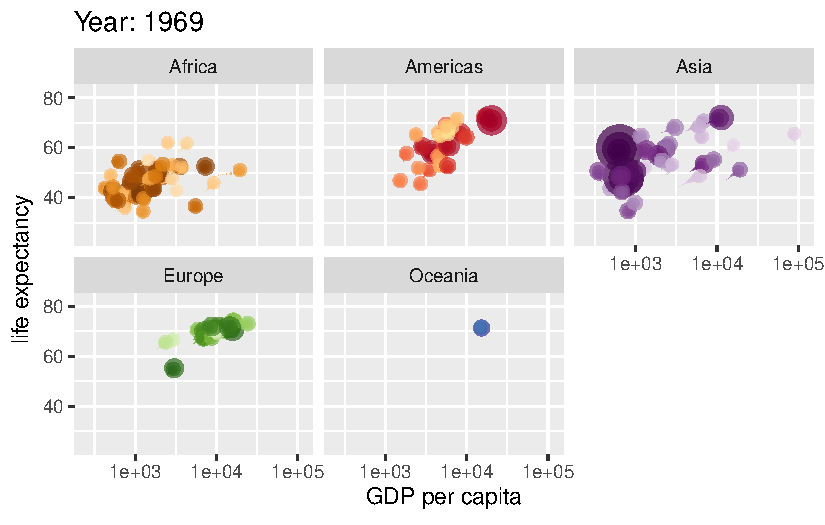
\includegraphics{class05_files/figure-pdf/unnamed-chunk-24-31.pdf}

}

\end{figure}

\begin{figure}[H]

{\centering 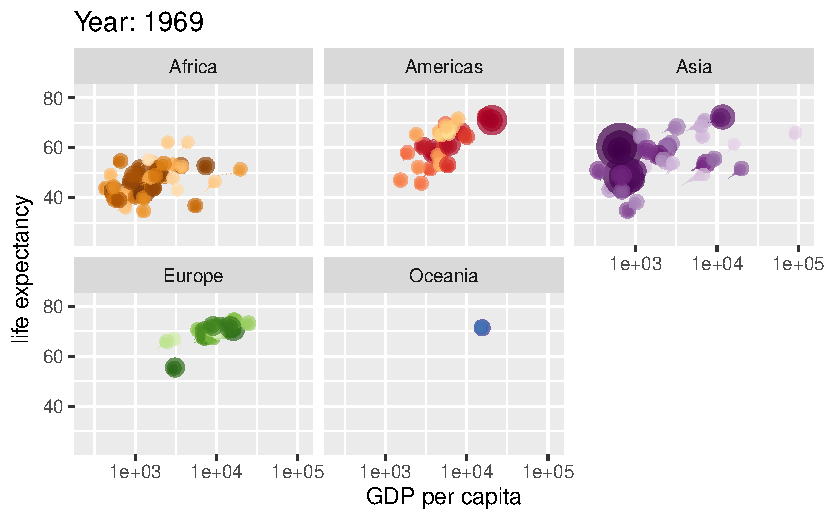
\includegraphics{class05_files/figure-pdf/unnamed-chunk-24-32.pdf}

}

\end{figure}

\begin{figure}[H]

{\centering 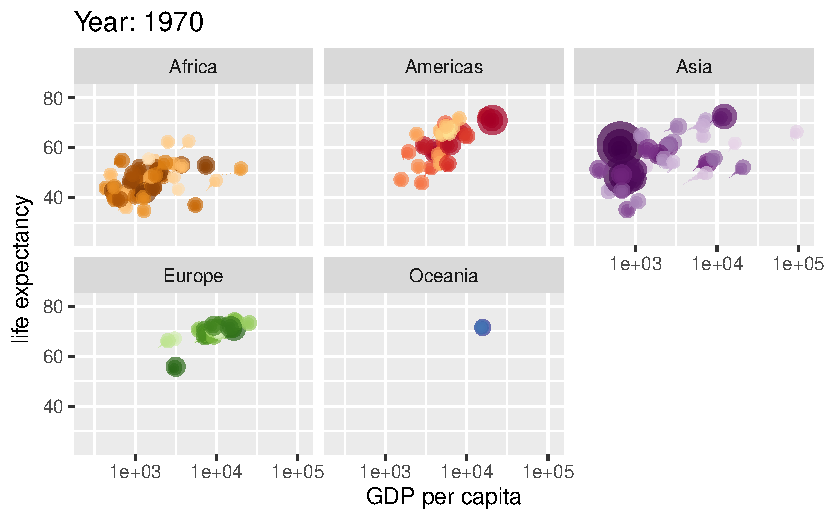
\includegraphics{class05_files/figure-pdf/unnamed-chunk-24-33.pdf}

}

\end{figure}

\begin{figure}[H]

{\centering 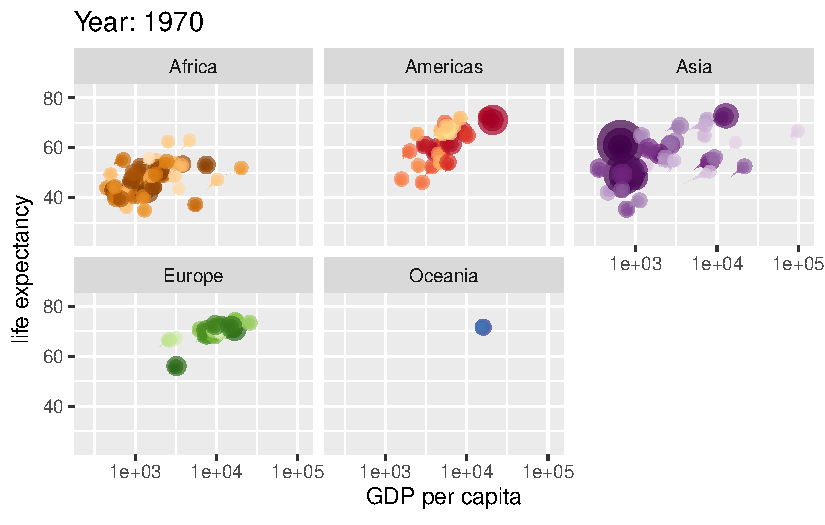
\includegraphics{class05_files/figure-pdf/unnamed-chunk-24-34.pdf}

}

\end{figure}

\begin{figure}[H]

{\centering 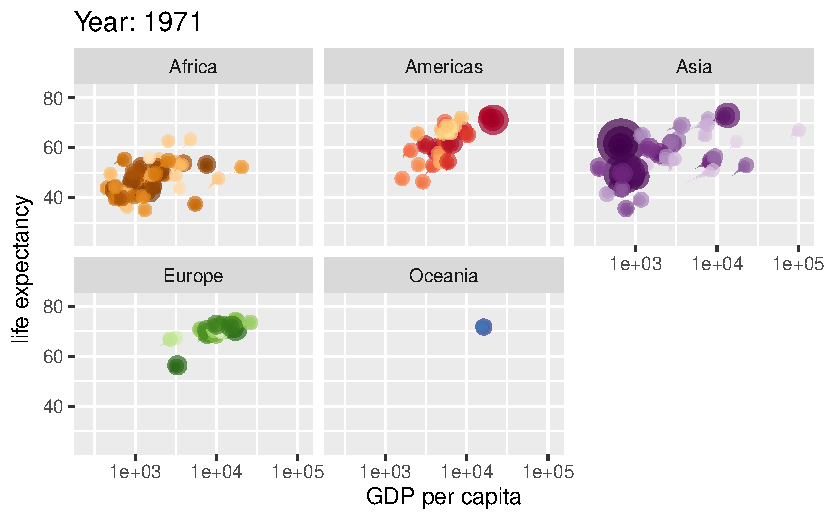
\includegraphics{class05_files/figure-pdf/unnamed-chunk-24-35.pdf}

}

\end{figure}

\begin{figure}[H]

{\centering \includegraphics{class05_files/figure-pdf/unnamed-chunk-24-36.pdf}

}

\end{figure}

\begin{figure}[H]

{\centering \includegraphics{class05_files/figure-pdf/unnamed-chunk-24-37.pdf}

}

\end{figure}

\begin{figure}[H]

{\centering \includegraphics{class05_files/figure-pdf/unnamed-chunk-24-38.pdf}

}

\end{figure}

\begin{figure}[H]

{\centering \includegraphics{class05_files/figure-pdf/unnamed-chunk-24-39.pdf}

}

\end{figure}

\begin{figure}[H]

{\centering \includegraphics{class05_files/figure-pdf/unnamed-chunk-24-40.pdf}

}

\end{figure}

\begin{figure}[H]

{\centering \includegraphics{class05_files/figure-pdf/unnamed-chunk-24-41.pdf}

}

\end{figure}

\begin{figure}[H]

{\centering \includegraphics{class05_files/figure-pdf/unnamed-chunk-24-42.pdf}

}

\end{figure}

\begin{figure}[H]

{\centering \includegraphics{class05_files/figure-pdf/unnamed-chunk-24-43.pdf}

}

\end{figure}

\begin{figure}[H]

{\centering \includegraphics{class05_files/figure-pdf/unnamed-chunk-24-44.pdf}

}

\end{figure}

\begin{figure}[H]

{\centering \includegraphics{class05_files/figure-pdf/unnamed-chunk-24-45.pdf}

}

\end{figure}

\begin{figure}[H]

{\centering \includegraphics{class05_files/figure-pdf/unnamed-chunk-24-46.pdf}

}

\end{figure}

\begin{figure}[H]

{\centering \includegraphics{class05_files/figure-pdf/unnamed-chunk-24-47.pdf}

}

\end{figure}

\begin{figure}[H]

{\centering \includegraphics{class05_files/figure-pdf/unnamed-chunk-24-48.pdf}

}

\end{figure}

\begin{figure}[H]

{\centering \includegraphics{class05_files/figure-pdf/unnamed-chunk-24-49.pdf}

}

\end{figure}

\begin{figure}[H]

{\centering \includegraphics{class05_files/figure-pdf/unnamed-chunk-24-50.pdf}

}

\end{figure}

\begin{figure}[H]

{\centering \includegraphics{class05_files/figure-pdf/unnamed-chunk-24-51.pdf}

}

\end{figure}

\begin{figure}[H]

{\centering \includegraphics{class05_files/figure-pdf/unnamed-chunk-24-52.pdf}

}

\end{figure}

\begin{figure}[H]

{\centering \includegraphics{class05_files/figure-pdf/unnamed-chunk-24-53.pdf}

}

\end{figure}

\begin{figure}[H]

{\centering \includegraphics{class05_files/figure-pdf/unnamed-chunk-24-54.pdf}

}

\end{figure}

\begin{figure}[H]

{\centering \includegraphics{class05_files/figure-pdf/unnamed-chunk-24-55.pdf}

}

\end{figure}

\begin{figure}[H]

{\centering \includegraphics{class05_files/figure-pdf/unnamed-chunk-24-56.pdf}

}

\end{figure}

\begin{figure}[H]

{\centering \includegraphics{class05_files/figure-pdf/unnamed-chunk-24-57.pdf}

}

\end{figure}

\begin{figure}[H]

{\centering \includegraphics{class05_files/figure-pdf/unnamed-chunk-24-58.pdf}

}

\end{figure}

\begin{figure}[H]

{\centering \includegraphics{class05_files/figure-pdf/unnamed-chunk-24-59.pdf}

}

\end{figure}

\begin{figure}[H]

{\centering \includegraphics{class05_files/figure-pdf/unnamed-chunk-24-60.pdf}

}

\end{figure}

\begin{figure}[H]

{\centering \includegraphics{class05_files/figure-pdf/unnamed-chunk-24-61.pdf}

}

\end{figure}

\begin{figure}[H]

{\centering \includegraphics{class05_files/figure-pdf/unnamed-chunk-24-62.pdf}

}

\end{figure}

\begin{figure}[H]

{\centering \includegraphics{class05_files/figure-pdf/unnamed-chunk-24-63.pdf}

}

\end{figure}

\begin{figure}[H]

{\centering \includegraphics{class05_files/figure-pdf/unnamed-chunk-24-64.pdf}

}

\end{figure}

\begin{figure}[H]

{\centering \includegraphics{class05_files/figure-pdf/unnamed-chunk-24-65.pdf}

}

\end{figure}

\begin{figure}[H]

{\centering \includegraphics{class05_files/figure-pdf/unnamed-chunk-24-66.pdf}

}

\end{figure}

\begin{figure}[H]

{\centering \includegraphics{class05_files/figure-pdf/unnamed-chunk-24-67.pdf}

}

\end{figure}

\begin{figure}[H]

{\centering \includegraphics{class05_files/figure-pdf/unnamed-chunk-24-68.pdf}

}

\end{figure}

\begin{figure}[H]

{\centering \includegraphics{class05_files/figure-pdf/unnamed-chunk-24-69.pdf}

}

\end{figure}

\begin{figure}[H]

{\centering \includegraphics{class05_files/figure-pdf/unnamed-chunk-24-70.pdf}

}

\end{figure}

\begin{figure}[H]

{\centering \includegraphics{class05_files/figure-pdf/unnamed-chunk-24-71.pdf}

}

\end{figure}

\begin{figure}[H]

{\centering \includegraphics{class05_files/figure-pdf/unnamed-chunk-24-72.pdf}

}

\end{figure}

\begin{figure}[H]

{\centering \includegraphics{class05_files/figure-pdf/unnamed-chunk-24-73.pdf}

}

\end{figure}

\begin{figure}[H]

{\centering \includegraphics{class05_files/figure-pdf/unnamed-chunk-24-74.pdf}

}

\end{figure}

\begin{figure}[H]

{\centering \includegraphics{class05_files/figure-pdf/unnamed-chunk-24-75.pdf}

}

\end{figure}

\begin{figure}[H]

{\centering \includegraphics{class05_files/figure-pdf/unnamed-chunk-24-76.pdf}

}

\end{figure}

\begin{figure}[H]

{\centering \includegraphics{class05_files/figure-pdf/unnamed-chunk-24-77.pdf}

}

\end{figure}

\begin{figure}[H]

{\centering \includegraphics{class05_files/figure-pdf/unnamed-chunk-24-78.pdf}

}

\end{figure}

\begin{figure}[H]

{\centering \includegraphics{class05_files/figure-pdf/unnamed-chunk-24-79.pdf}

}

\end{figure}

\begin{figure}[H]

{\centering \includegraphics{class05_files/figure-pdf/unnamed-chunk-24-80.pdf}

}

\end{figure}

\begin{figure}[H]

{\centering \includegraphics{class05_files/figure-pdf/unnamed-chunk-24-81.pdf}

}

\end{figure}

\begin{figure}[H]

{\centering \includegraphics{class05_files/figure-pdf/unnamed-chunk-24-82.pdf}

}

\end{figure}

\begin{figure}[H]

{\centering \includegraphics{class05_files/figure-pdf/unnamed-chunk-24-83.pdf}

}

\end{figure}

\begin{figure}[H]

{\centering \includegraphics{class05_files/figure-pdf/unnamed-chunk-24-84.pdf}

}

\end{figure}

\begin{figure}[H]

{\centering \includegraphics{class05_files/figure-pdf/unnamed-chunk-24-85.pdf}

}

\end{figure}

\begin{figure}[H]

{\centering \includegraphics{class05_files/figure-pdf/unnamed-chunk-24-86.pdf}

}

\end{figure}

\begin{figure}[H]

{\centering \includegraphics{class05_files/figure-pdf/unnamed-chunk-24-87.pdf}

}

\end{figure}

\begin{figure}[H]

{\centering \includegraphics{class05_files/figure-pdf/unnamed-chunk-24-88.pdf}

}

\end{figure}

\begin{figure}[H]

{\centering \includegraphics{class05_files/figure-pdf/unnamed-chunk-24-89.pdf}

}

\end{figure}

\begin{figure}[H]

{\centering \includegraphics{class05_files/figure-pdf/unnamed-chunk-24-90.pdf}

}

\end{figure}

\begin{figure}[H]

{\centering \includegraphics{class05_files/figure-pdf/unnamed-chunk-24-91.pdf}

}

\end{figure}

\begin{figure}[H]

{\centering \includegraphics{class05_files/figure-pdf/unnamed-chunk-24-92.pdf}

}

\end{figure}

\begin{figure}[H]

{\centering \includegraphics{class05_files/figure-pdf/unnamed-chunk-24-93.pdf}

}

\end{figure}

\begin{figure}[H]

{\centering \includegraphics{class05_files/figure-pdf/unnamed-chunk-24-94.pdf}

}

\end{figure}

\begin{figure}[H]

{\centering \includegraphics{class05_files/figure-pdf/unnamed-chunk-24-95.pdf}

}

\end{figure}

\begin{figure}[H]

{\centering \includegraphics{class05_files/figure-pdf/unnamed-chunk-24-96.pdf}

}

\end{figure}

\begin{figure}[H]

{\centering \includegraphics{class05_files/figure-pdf/unnamed-chunk-24-97.pdf}

}

\end{figure}

\begin{figure}[H]

{\centering \includegraphics{class05_files/figure-pdf/unnamed-chunk-24-98.pdf}

}

\end{figure}

\begin{figure}[H]

{\centering \includegraphics{class05_files/figure-pdf/unnamed-chunk-24-99.pdf}

}

\end{figure}

\begin{figure}[H]

{\centering \includegraphics{class05_files/figure-pdf/unnamed-chunk-24-100.pdf}

}

\end{figure}

\hypertarget{happy-cat}{%
\section{Happy Cat}\label{happy-cat}}

\includegraphics{class05_files/mediabag/giphy-downsized-larg.gif}



\end{document}
